% !TeX program = pdflatex
\documentclass[11pt,a4paper,oneside]{report}             % Single-side
%\documentclass[11pt,a4paper,twoside,openright]{report}  % Duplex

\usepackage{ifxetex}
\ifxetex
  \usepackage{fontspec}
\else
  \usepackage[T1]{fontenc}
  \usepackage[utf8]{inputenc}
  \usepackage{lmodern}
\fi

\usepackage[english,magyar]{babel} % Alapértelmezés szerint utoljára definiált nyelv lesz aktív, de később külön beállítjuk az aktív nyelvet.

\usepackage{cmap}
\usepackage{amsfonts,amsmath,amssymb} % Mathematical symbols.
\usepackage[ruled,boxed,resetcount,linesnumbered]{algorithm2e} % For pseudocodes.
\usepackage{booktabs} % For publication quality tables for LaTeX
\usepackage{graphicx}


%\usepackage{fancyhdr}
%\usepackage{lastpage}

\usepackage{anysize}
\usepackage{sectsty}
\usepackage{setspace}  % Ettol a tablazatok, abrak, labjegyzetek maradnak 1-es sorkozzel!

\usepackage{hyperref} % For hyperlinks in the generated document. 
\usepackage{color}
\usepackage{listings} % For source code snippets.

\usepackage[amsmath,thmmarks]{ntheorem} % Theorem-like environments.

\usepackage[hang]{caption}





%%--------------------------------------------------------------------------------------
% Elnevezések
%--------------------------------------------------------------------------------------
\newcommand{\dolgozatnyelve}{\selectlanguage{magyar}}

\newcommand{\bme}{Budapesti Műszaki és Gazdaságtudományi Egyetem}
\newcommand{\vik}{Villamosmérnöki és Informatikai Kar}

\newcommand{\bmemit}{Méréstechnika és Információs Rendszerek Tanszék}

\newcommand{\keszitette}{Készítette}
\newcommand{\konzulens}{Konzulens}

\newcommand{\bsc}{Szakdolgozat}
\newcommand{\msc}{Diplomaterv}

\newcommand{\pelda}{Példa}
\newcommand{\definicio}{Definíció}
\newcommand{\tetel}{Tétel}

\newcommand{\bevezeto}{Bevezető}
\newcommand{\koszonetnyilvanitas}{Köszönetnyilvánítás}
\newcommand{\abrakjegyzeke}{Ábrák jegyzéke}
\newcommand{\tablazatokjegyzeke}{Táblázatok jegyzéke}
\newcommand{\irodalomjegyzek}{Irodalomjegyzék}
\newcommand{\fuggelek}{Függelék}

\newcommand{\szerzo}{\vikszerzoVezeteknev{} \vikszerzoKeresztnev}


\newcommand{\englishParagraph}{
	\setlength{\parindent}{0em} % angol nyelvű dokumentumokban jellemző
	\setlength{\parskip}{0.5em} % angol nyelvű dokumentumokban jellemző
	\nonfrenchspacing
}

\newcommand{\hungarianParagraph}{
	\setlength{\parindent}{2em} % angol nyelvű dokumentumokban jellemző
	\setlength{\parskip}{0em}   % angol nyelvű dokumentumokban jellemző
	\frenchspacing
}

\newcommand{\defaultParagraph}{
	\hungarianParagraph
}

\bibliographystyle{huplain}
  % Beállítások magyar nyelvű dolgozathoz
%--------------------------------------------------------------------------------------
% Elnevezések
%--------------------------------------------------------------------------------------
\newcommand{\dolgozatnyelve}{\selectlanguage{english}}

\newcommand{\bme}{Budapest University of Technology and Economics}
\newcommand{\vik}{Faculty of Electrical Engineering and Informatics}

\newcommand{\bmemit}{Department of Measurement and Information Systems}

\newcommand{\keszitette}{Author}
\newcommand{\konzulens}{Advisor}

\newcommand{\bsc}{Bachelor's Thesis}
\newcommand{\msc}{Master's Thesis}

\newcommand{\pelda}{Example}
\newcommand{\definicio}{Definition}
\newcommand{\tetel}{Theorem}

\newcommand{\bevezeto}{Introduction}
\newcommand{\koszonetnyilvanitas}{Acknowledgements}
\newcommand{\abrakjegyzeke}{List of Figures}
\newcommand{\tablazatokjegyzeke}{List of Tables}
\newcommand{\irodalomjegyzek}{Bibliography}
\newcommand{\fuggelek}{Appendix}

\newcommand{\szerzo}{\vikszerzoKeresztnev{} \vikszerzoVezeteknev}

\newcommand{\englishParagraph}{
	\setlength{\parindent}{0em} % angol nyelvű dokumentumokban jellemző
	\setlength{\parskip}{0.5em} % angol nyelvű dokumentumokban jellemző
	\nonfrenchspacing
	\renewcommand{\figureautorefname}{Figure}
	\renewcommand{\tableautorefname}{Table}
	\renewcommand{\partautorefname}{Part}
	\renewcommand{\chapterautorefname}{Chapter}
	\renewcommand{\sectionautorefname}{Section}
	\renewcommand{\subsectionautorefname}{Section}
	\renewcommand{\subsubsectionautorefname}{Section}
}


\newcommand{\hungarianParagraph}{
	\setlength{\parindent}{2em} % angol nyelvű dokumentumokban jellemző
	\setlength{\parskip}{0em}   % angol nyelvű dokumentumokban jellemző
	\frenchspacing
}

\newcommand{\defaultParagraph}{
	\englishParagraph
}

\newcommand{\ie}{i.e.\@\xspace}
\newcommand{\Ie}{I.e.\@\xspace}
\newcommand{\eg}{e.g.\@\xspace}
\newcommand{\Eg}{E.g.\@\xspace}
\newcommand{\etal}{et al.\@\xspace}
\newcommand{\etc}{etc.\@\xspace}

\bibliographystyle{plain}
 % Settings for English documents

%--------------------------------------------------------------------------------------
% Main variables


%--------------------------------------------------------------------------------------
\newcommand{\vikszerzoVezeteknev}{Kővári}
\newcommand{\vikszerzoKeresztnev}{Zsolt}
\newcommand{\vikkonzulensA}{Gábor Szárnyas} % Első konzulens neve
\newcommand{\vikkonzulensB}{Dr. István Ráth} % Második konzulens neve; hagyd üresen, ha egy konzulensed van.
\newcommand{\vikcim}{Performance Analysis of Graph Queries} % Cím
\newcommand{\viktanszek}{\bmemit} % Tanszék
\newcommand{\vikdoktipus}{} % Dokumentum típusa (diplomaterv, szakdolgozat, TDK-dolgozat, stb.)

%--------------------------------------------------------------------------------------
% TDK-specifikus változók
%--------------------------------------------------------------------------------------
\newcommand{\tdkszerzoB}{} % Második szerző neve; hagyd üresen, ha egyedül í­rtad a TDK-t.
\newcommand{\tdkev}{2015} % A dolgozat írásának éve (pl. "2014") (Ez OTDK-nál eltérhet az aktuális évtől.)

% További adatok az OTDK címlaphoz (BME-s TDK-hoz nem kell kitölteni)
\newcommand{\tdkevfolyamA}{IV} % Első szerző évfolyama, római számmal (pl. IV).
\newcommand{\tdkevfolyamB}{III} % Második szerző évfolyama, római számmal (pl. III).
\newcommand{\tdkkonzulensbeosztasA}{egyetemi tanár} % Első konzulens beosztása (pl. egyetemi docens)
\newcommand{\tdkkonzulensbeosztasB}{doktorandusz} % Második konzulens beosztása (pl. egyetemi docens)
\newcommand{\szerzoMeta}{\vikszerzoVezeteknev{} \vikszerzoKeresztnev} % egy szerző esetén
%\newcommand{\szerzoMeta}{\vikszerzoVezeteknev{} \vikszerzoKeresztnev, \tdkszerzoB} % két szerző esetén

%--------------------------------------------------------------------------------------
% Page layout setup
%--------------------------------------------------------------------------------------
% we need to redefine the pagestyle plain
% another possibility is to use the body of this command without \fancypagestyle
% and use \pagestyle{fancy} but in that case the special pages
% (like the ToC, the References, and the Chapter pages)remain in plane style

\pagestyle{plain}
\marginsize{35mm}{25mm}{15mm}{15mm}

\setcounter{secnumdepth}{0}
\sectionfont{\large\upshape\bfseries}
\setcounter{secnumdepth}{2}

\sloppy % Margón túllógó sorok tiltása.
\widowpenalty=10000 \clubpenalty=10000 %A fattyú- és árvasorok elkerülése
\def\hyph{-\penalty0\hskip0pt\relax} % Kötőjeles szavak elválasztásának engedélyezése


%--------------------------------------------------------------------------------------
% Setup hyperref package
%--------------------------------------------------------------------------------------
\hypersetup{
    bookmarks=true,            % show bookmarks bar?
    unicode=false,              % non-Latin characters in Acrobat's bookmarks
    pdftitle={\vikcim},        % title
    pdfauthor={\szerzoMeta},    % author
    pdfsubject={\vikdoktipus}, % subject of the document
    pdfcreator={\szerzoMeta},   % creator of the document
    pdfproducer={},    % producer of the document
    pdfkeywords={},    % list of keywords (separate then by comma)
    pdfnewwindow=true,         % links in new window
    colorlinks=true,           % false: boxed links; true: colored links
    linkcolor=black,           % color of internal links
    citecolor=black,           % color of links to bibliography
    filecolor=black,           % color of file links
    urlcolor=black             % color of external links
}


%--------------------------------------------------------------------------------------
% Set up listings
%--------------------------------------------------------------------------------------
\definecolor{lightgray}{rgb}{0.95,0.95,0.95}
\lstset{
	basicstyle=\scriptsize\ttfamily, % print whole listing small
	keywordstyle=\color{black}\bfseries, % bold black keywords
	identifierstyle=, % nothing happens
	commentstyle=\color{green}, % green comments
	stringstyle=\scriptsize,
	showstringspaces=false, % no special string spaces
	aboveskip=3pt,
	belowskip=3pt,
	backgroundcolor=\color{lightgray},
	columns=flexible,
	keepspaces=true,
	escapeinside={(*@}{@*)},
	literate=*
		{á}{{\'a}}1	{é}{{\'e}}1	{í}{{\'i}}1	{ó}{{\'o}}1	{ö}{{\"o}}1	{ő}{{\H{o}}}1	{ú}{{\'u}}1	{ü}{{\"u}}1	{ű}{{\H{u}}}1
		{Á}{{\'A}}1	{É}{{\'E}}1	{Í}{{\'I}}1	{Ó}{{\'O}}1	{Ö}{{\"O}}1	{Ő}{{\H{O}}}1	{Ú}{{\'U}}1	{Ü}{{\"U}}1	{Ű}{{\H{U}}}1
} 	
\def\lstlistingname{lista}	


%--------------------------------------------------------------------------------------
% Set up theorem-like environments
%--------------------------------------------------------------------------------------
% Using ntheorem package -- see http://www.math.washington.edu/tex-archive/macros/latex/contrib/ntheorem/ntheorem.pdf

\theoremstyle{plain}
\theoremseparator{.}
\newtheorem{example}{\pelda}

\theoremseparator{.}
%\theoremprework{\bigskip\hrule\medskip}
%\theorempostwork{\hrule\bigskip}
\theorembodyfont{\upshape}
\theoremsymbol{{\large \ensuremath{\centerdot}}}
\newtheorem{definition}{\definicio}

\theoremseparator{.}
%\theoremprework{\bigskip\hrule\medskip}
%\theorempostwork{\hrule\bigskip}
\newtheorem{theorem}{\tetel}


%--------------------------------------------------------------------------------------
% Some new commands and declarations
%--------------------------------------------------------------------------------------
\newcommand{\code}[1]{{\upshape\ttfamily\scriptsize\indent #1}}
\newcommand{\doi}[1]{DOI: \href{http://dx.doi.org/\detokenize{#1}}{\raggedright{\texttt{\detokenize{#1}}}}} % A hivatkozások közt így könnyebb DOI-t megadni.

\newcommand{\CC}{C\nolinebreak\hspace{-.05em}\raisebox{.4ex}{\tiny\bf +}\nolinebreak\hspace{-.10em}\raisebox{.4ex}{\tiny\bf +}}

\DeclareMathOperator*{\argmax}{arg\,max}
%\DeclareMathOperator*[1]{\floor}{arg\,max}
\DeclareMathOperator{\sign}{sgn}
\DeclareMathOperator{\rot}{rot}


%--------------------------------------------------------------------------------------
% Setup captions
%--------------------------------------------------------------------------------------
\captionsetup[figure]{
	width=.75\textwidth,
	aboveskip=10pt}

\renewcommand{\captionlabelfont}{\bf}
%\renewcommand{\captionfont}{\footnotesize\it}


%--------------------------------------------------------------------------------------
% Redefine reference style
%--------------------------------------------------------------------------------------
\newcommand{\figref}[1]{\ref{fig:#1}.}
\renewcommand{\eqref}[1]{(\ref{eq:#1})}
\newcommand{\listref}[1]{\ref{listing:#1}.}
\newcommand{\sectref}[1]{\ref{sect:#1}}
\newcommand{\tabref}[1]{\ref{tab:#1}.}


%--------------------------------------------------------------------------------------
% Hyphenation exceptions
%--------------------------------------------------------------------------------------
\hyphenation{Shakes-peare Mar-seilles ár-víz-tű-rő tü-kör-fú-ró-gép}


\author{\vikszerzo}
\title{\viktitle}


%--------------------------------------------------------------------------------------
% Table of contents and the main text
%--------------------------------------------------------------------------------------
\begin{document}



%~~~~~~~~~~~~~~~~~~~~~~~~~~~~~~~~~~~~~~~~~~~~~~~~~~~~~~~~~~~~~~~~~~~~~~~~~~~~~~~~~~~~~~


\pagenumbering{gobble}
\dolgozatnyelve
\englishParagraph
\singlespacing
%%--------------------------------------------------------------------------------------
% Feladatkiiras (a tanszeken atveheto, kinyomtatott valtozat)
%--------------------------------------------------------------------------------------
\clearpage
\begin{center}
\large
\textbf{FELADATKIÍRÁS}\\
\end{center}

A feladatkiírást a tanszéki adminisztrációban lehet átvenni, és a leadott munkába eredeti, tanszéki pecséttel ellátott és a tanszékvezető által aláírt lapot kell belefűzni (ezen oldal \emph{helyett}, ez az oldal csak útmutatás). Az elektronikusan feltöltött dolgozatban már nem kell beleszerkeszteni ezt a feladatkiírást.

\onehalfspacing
\defaultParagraph



%~~~~~~~~~~~~~~~~~~~~~~~~~~~~~~~~~~~~~~~~~~~~~~~~~~~~~~~~~~~~~~~~~~~~~~~~~~~~~~~~~~~~~~
	%%--------------------------------------------------------------------------------------
%	The title page
%--------------------------------------------------------------------------------------
\begin{titlepage}
\begin{center}

\includegraphics[width=60mm,keepaspectratio]{figures/bme_logo.pdf}\\
\vspace{0.3cm}
\textbf{\bme}\\
\textmd{\vik}\\
\textmd{\viktanszek}\\[5cm]

\vspace{0.4cm}
{\huge \bfseries \vikcim}\\[0.8cm]
\vspace{0.5cm}
\textsc{\Large \vikdoktipus}\\[4cm]

{
	\renewcommand{\arraystretch}{0.85}
	\begin{tabular}{cc}
	 \makebox[7cm]{\emph{\keszitette}} & \makebox[7cm]{\emph{\konzulens}} \\ \noalign{\smallskip}
	 \makebox[7cm]{\szerzo} & \makebox[7cm]{\vikkonzulensA} \\
	  & \makebox[7cm]{\vikkonzulensB} \\
	\end{tabular}
}

\vfill
{\large \today}
\end{center}
\end{titlepage}


		   % Szakdolgozat/Diplomaterv címlap
	%% TDK címlap
\begin{titlepage}
  \begin{center}  
  
\includegraphics[width=7cm]{./figures/bme_logo.pdf}
  \vspace{0.3cm}
  
  \bme \\
  \vik \\
  \viktanszek \\
  \vspace{5cm}
  
  \huge {\vikcim}
  \vspace{1.5cm}
  
  \large {\textbf{\vikdoktipus}}
  \vfill
    
  {\Large 
  	\keszitette: \\ \vspace{0.3cm}
  	\szerzo \\
  	\vspace{1.5cm}
  	\konzulens: \\ \vspace{0.3cm}
  	\vikkonzulensA \\
  	\vikkonzulensB \\
  }
  
  \vspace{2cm}
  \large {\tdkev.}
 \end{center}
\end{titlepage}
%% Címlap vége	% TDK címlap
	%%% OTDK külső címlap
\begin{titlepage}
  	$\;$ 
	\vspace{5cm}
	
	\begin{center}
	\Huge
	\textbf{TDK-dolgozat}\let\thefootnote\relax\footnote{A dolgozat bemutatását a XXXXXXXXX  ``Lorem ipsum dolor sit amet'' című program támogatta.}
	\end{center}
	
	\vspace{13cm}
	
	\Large
	\hspace{8cm} \szerzo
	
	\hspace{8cm} \tdkszerzoB
	
	\hspace{8cm} \tdkev.
\end{titlepage}

\newpage
\thispagestyle{empty}


%% OTDK belső címlap
\begin{titlepage}
  \begin{center}  
  
\includegraphics[width=7cm]{./figures/bme_logo.pdf}
  \vspace{0.3cm}
  
  \bme \\
  \vik \\
  \viktanszek \\
  \vspace{3.5cm}
  
  \huge {\vikcim}
  \vspace{1.5cm}
  
  \large {\textbf{\vikdoktipus}}
  \vfill
    
  {\Large 
  	{\large \keszitette:} \\ \vspace{0.2cm}
  	\szerzo \\ \tdkevfolyamA. évfolyam \\
	\vspace{0.5cm}
	\tdkszerzoB \\ \tdkevfolyamB. évfolyam \\
  	\vspace{1.5cm}
  	{\large \konzulens:} \\ \vspace{0.2cm}
  	\vikkonzulensA,\\ \tdkkonzulensbeosztasA \\
  	\vspace{0.5cm}
  	\vikkonzulensB,\\ \tdkkonzulensbeosztasB \\
  }
  
  \vspace{2cm}
  \large {\tdkev.}
  
 \end{center}
\end{titlepage}   % OTDK címlap
 

% Table of Contents
%~~~~~~~~~~~~~~~~~~~~~~~~~~~~~~~~~~~~~~~~~~~~~~~~~~~~~~~~~~~~~~~~~~~~~~~~~~~~~~~~~~~~~~
	\tableofcontents\vfill


% Declaration and Abstract
%~~~~~~~~~~~~~~~~~~~~~~~~~~~~~~~~~~~~~~~~~~~~~~~~~~~~~~~~~~~~~~~~~~~~~~~~~~~~~~~~~~~~~~
	\pagenumbering{roman}
\setcounter{page}{1}

\selectlanguage{magyar}
%\hungarianParagraph

\englishParagraph
%----------------------------------------------------------------------------
% Abstract in Hungarian
%----------------------------------------------------------------------------
\chapter*{Kivonat}\addcontentsline{toc}{chapter}{Kivonat}

A gráf alapú adatmodellező, illetve adatbázis-kezelő keretrendszerek esetén kulcsfontosságú a minél nagyobb teljesítmény, illetve rövidebb válaszidő biztosítása, különösen az olyan alkalmazási területeken, ahol egyszerre több, strukturálisan összetett lekérdezést kell újra és újra kiértékelni egy folyamatosan változó (gráf)adatstruktúra felett. A modern, relációs adatmodellt elvető NoSQL technológiák terjedésével egyre nagyobb figyelmet kap az ilyen rendszerek teljesítőképessége és skálázhatósága, így az utóbbi években több olyan benchmark is megjelent, melynek fő célja az ilyen rendszerek teljesítőképességének, különösen a lekérdezések skálázhatóságának szisztematikus kiértékelése. 

A legtöbb mérési keretrendszer számításba vesz bemenet és teljesítmény leíró metrikákat, mint például a gráf csomópontjainak száma vagy a lekérdezések válaszideje, ugyanakkor nagyon nehéz az eredmények összehasonlítása, mert a méréshez használt bemenetek (gráfok, lekérdezések komplexitása, illetve a gráfon a mérés során végrehajtott változtatások jellege, összességében a \emph{terhelési profil}) igen nagy méret- és tulajdonságbeli eltéréseket mutatnak - ezekről pedig megelőző kutatási eredmények kimutatták, hogy jelentős és változó mértékben befolyásolhatják az egyes eszközök viselkedését, teljesítménykarakterisztikáját.
% Azonban, ezen keretrendszerek nem veszik figyelembe a gráf belső hálózatán végbemenő változásokat, és kizárólag egy struktúrájú gráfra koncentrálnak. 

A jelen dolgozat elsődleges célja, hogy - korábbi kutatásokat folytatva - kidolgozzon egy olyan mérési módszertant és hozzá kapcsolódó keretrendszert, amelynek segítségével a gráf alapú adatbázis-kezelő rendszerek teljesítménybeli összehasonlítása szisztematikusan és reprodukálhatóan hajtható végre. Fő eredményként a teljesítménymérés céljára különböző gráf topológiákat javasolunk, amelyek jellemzésére gráfmetrikákat definiálunk. A metrikák segítségével jellemezhető az egyes mérések nehézsége, illetve bizonyos eszközök esetén kapcsolatot is találhatunk a gráfokat jellemző metrikák és a lekérdezések futásidői között. A módszertan és a keretrendszer képességeinek bemutatására a dolgozat bemutat egy komplex esettanulmányt, mely magába foglalja számos kísérlet automatizált elvégzését és magasszintű statisztikai analízis eszközökkel támogatott kiértékelését is.

%, így metrikáink később felhasználhatóak a gráflekérdezések optimalizálása - jelenleg még nagyon kiforratlan - területén. 



\vfill
\selectlanguage{english}
\englishParagraph


%----------------------------------------------------------------------------
% Abstract in English
%----------------------------------------------------------------------------
\chapter*{Abstract}\addcontentsline{toc}{chapter}{Abstract}
Achieving high-performance query evaluation represents a crucial problem in modern graph-based database systems. The response time of the query evaluation on a graph is affected by the complexity of the particular query and the underlying network structure of the graph. 

Several state-of-the-art benchmark frameworks exist that assess the performance and correctness of query evaluations as they create real world-like workloads and define suites of systematic queries. However, these benchmark frameworks rely on only one particular type of network and they do not concentrate on a significant alteration of the underlying graph. Although most of them define metrics for characterizing the specific aspects of performance (response time, query evaluations per hour, etc.), most of them lack such comprehensive metrics for the queries and the graph.
As a consequence, they cannot determine the correlations between workload and performance.

%Due to the absence of metrics, it is difficult to give a precise characterization of the complexity for various benchmarks. Hence, it is difficult %to compare the benchmarks and the published results to each other.

In order to provide solid foundations to characterize the complexity of graph benchmarks, we elaborate a benchmark framework for graph-based database systems.

We use various graph metrics to describe the structure of the graph %create regression models to determine the relationships quantitatively.
and use a varied set of graph topologies for benchmarking. This will allow us to perform in-depth analysis on the relationships between the structure of the graph in the database and the performance of the query evaluations. These results can be used to obtain advanced heuristics for the optimization of graph query engines. While the optimization of relational databases has well-known techniques documented by a wide literature, the problem for graph query engines is yet be discussed thoroughly.




%The performance of query evaluations depends on the topology of the model, and the complexity of the particular query. Our primary goal is that --- %by defining model and query-related quantitative metrics ---  to find a considerable connection between metrics and the performance, and thus, be %able to predict the query evaluation time.

%Based on the metrics and their effect to the performance, we are able to make decisions in design to achieve on the optimal performance. %Furthermore, this knowledge can be utilized in the area of real-time query optimization engines as well.

%We investigate various NoSQL database systems via regression analysis in order to find different model-related metrics that are suited to %characterize their performance appropriately. Based on a real model, we generate graphs with various topologies and distributions to find metrics %from different aspects.

%Furthermore, we explore that whether an arbitrarily structured model's performance is predictable via our regression analysis, and also predict %which database system from our scope can be associated to the model in order to achieve an optimal performance.

%Finally, being motivated by the real-time optimization engines, we search answers whether by reducing the cost of metric calculations, an arbitrary %model's performance is still predictable.


\vfill
\dolgozatnyelve
\defaultParagraph

\newcounter{romanPage}
\setcounter{romanPage}{\value{page}}
\stepcounter{romanPage}	  %TODO Összefoglaló -- TDK és OTDK esetén nem kötelező


% The main part of the thesis
%~~~~~~~~~~~~~~~~~~~~~~~~~~~~~~~~~~~~~~~~~~~~~~~~~~~~~~~~~~~~~~~~~~~~~~~~~~~~~~~~~~~~~~
\pagenumbering{arabic}

	%\newpage
\begin{enumerate}
	\item \textbf{Introduction}
	\begin{enumerate}[label*=\arabic*.]
		\item \textbf{Problem}
		\item \textbf{Concepts}
			\item \textbf{Contributions}
			\item \textbf{Structure of the Report}
		\end{enumerate}
		\item \textbf{Background}
		\begin{enumerate}[label*=\arabic*.]
			\item \textbf{NoSQL}
			\item \textbf{RDF}
			\item \textbf{Statistics}
			\begin{enumerate}[label*=\arabic*.]
				\item \textit{Population and Sample}
				\item \textit{Distributions}
				\item \textit{Correlation}
				\item \textit{Regression}
			\end{enumerate}
			\item \textbf{Graph Theory}
			\begin{enumerate}[label*=\arabic*.]
				\item \textit{Metrics}
				\item \textit{Random-Graph}
				\item \textit{Scale-Free}
				\item \textit{Watts-Strogatz}
				\item \textit{Hierarchical}
			\end{enumerate}
		\end{enumerate}
	
	
	\item \textbf{Related Works}
	\begin{enumerate}[label*=\arabic*.]
		\item \textbf{Graph Analysis}
		\begin{enumerate}[label*=\arabic*.]
			\item \textit{Studies of Barabási and Albert}
			\item \textit{Network Robustness and Metric Correlations}
			\item \textit{Chinese Network Analysis}
			\item \textit{Conclusion}
		\end{enumerate}
		\item \textbf{NoSQL Benchmarks} or RDF / SPARQL Benchmarks
		\begin{enumerate}[label*=\arabic*.]
			\item \textit{YCSB}: maybe its not necessary
			\item \textit{Berlin}
			\item \textit{DBpedia}
			\item \textit{SP2}
			\item \textit{Conclusion}
		\end{enumerate}
	\end{enumerate}
	
	
	
	\item \textbf{Train Benchmark Framework}
	\begin{enumerate}[label*=\arabic*.]
		\item \textbf{Main Concepts}
		\item \textbf{Workflow}
		\item \textbf{The Domain}
		\item \textbf{Supported Formats}
		\item \textbf{Performance Comparison and Uniformity}
		\item \textbf{Tools}
		\item \textbf{Framework's Architecture}
	\end{enumerate}

	
	\item \textbf{Contributions}
	\begin{enumerate}[label*=\arabic*.]
		\item \textbf{Disadvantages of the Train Benchmark Domain} (necessary?)
		\item \textbf{A Real-life Model}
		\begin{enumerate}[label*=\arabic*.]
			\item \textit{Overview of a real-life Data: Train Schedules}
			\item \textit{Mapping to a Model}
			\item \textit{Model Analysis}
		\end{enumerate}
		\item \textbf{Extending the Framework with Analysis}
		\begin{enumerate}[label*=\arabic*.]
			\item \textit{Metrics Calculation}
			\item \textit{The New Architecture of the Framework}
			\item \textit{Workflow}
			\item \textit{Regression Analysis}
		\end{enumerate}
		\item \textbf{Model Generation}
		\begin{enumerate}[label*=\arabic*.]
			\item \textit{Concepts}
			\item \textit{Overall of the Generation Steps}
			\item \textit{Step 1: Topologies} (maybe omit "Step 1" from the title, it's strange)
			\begin{enumerate}[label*=\arabic*.]
				\item Random Graph
				\item Watts-Strogatz Model
				\item Scale-free Networks of Barabási-Albert
				\item Hierarchical Network
			\end{enumerate}
			\item \textit{Step 2: Schedule Connections}
			\item \textit{Possible Model Configurations}
			\item \textit{Uniform Model Generation}
		\end{enumerate}
		\item \textbf{The Workloads for Graph Queries Analysis}
		\begin{enumerate}[label*=\arabic*.]
			\item \textit{Main Goal}
			\item \textit{Sample Choosing}
			\begin{enumerate}[label*=\arabic*.]
				\item A Sample Based on Topologies
				\item A Sample Based on Metrics
			\end{enumerate}
			
			\item \textit{Model Configuration}
			\item \textit{Evaluated Queries}
			\item \textit{Test the Performance Estimation}
			\item \textit{Investigated Tools}
		\end{enumerate}
	\end{enumerate}
	
	
	\item \textbf{Evaluation}
	\begin{enumerate}[label*=\arabic*.]
		\item \textbf{Benchmarking Environment}
		\item \textbf{How to Read the Charts}
		\item \textbf{Multiple Regression Analysis}
		\item \textbf{MARS Analysis}
		\item \textbf{Performance Estimation}
		\item \textbf{Conclusions}
	\end{enumerate}
	\item \textbf{Summary}
	\begin{enumerate}[label*=\arabic*.]
		\item \textbf{Future Work}
	\end{enumerate}
	\item \textbf{Acknowledges}
\end{enumerate}






\newpage
\begin{enumerate}
	\item \textbf{Introduction}
		\begin{enumerate}[label*=\arabic*.]
			\item \textbf{Problem}\\
			In model oriented systems (not MDSD), performance is a key role.
			Databases, NoSQL systems -> increasing data -> importance of optimization.\\
			
			performance depends on workloads -> a bit different model + query implicate a high deviation in performance\\
			Real-time response. Important to estimate response time to optimize.
			
			There is no benchmark framework for NoSQL / RDF that investigates workload and performance relationship precisely, they only concentrate on performance. Only one static model can be found in these frameworks.
			

			\item \textbf{Concepts}\\
			A framework that systematically assess and analyze performance.
			Why is it good: utilizations in query optimizers.
	
			+ \textbf{\textbf{Fig}}: show the typical workflow of our goal: \\
			The challenge is to find regression models. \\
			Analyze models by descriptive metrics -> find connections.
			
			\item \textbf{Contributions}\\
			A brief overview of the work -> graph topologies with different distributions based on a real model-> metrics -> analyze performance, estimation\\
			Regression analysis.
			
			Arbitrary size, topology, density, and cardinality on the generated models.
			
			Test the framework's usability, test the performance estimation: arbitrary workload -> try to match a regression model. Can it be used in optimizations?
			\item \textbf{Structure of the Paper}
		\end{enumerate}
	\item \textbf{Background}
		\begin{enumerate}[label*=\arabic*.]
			\item \textbf{NoSQL} - briefly
			\item \textbf{RDF} - short, maybe 1 \textbf{\textbf{Fig}} of an example
			\item \textbf{Statistics}
				\begin{enumerate}[label*=\arabic*.]
					\item \textit{Population and Sample} - or sample only
					\item \textit{Distributions}\\ implicate the definition of random variable.
							Uniform; (normal?); poisson; pareto - power-law
					\item \textit{Correlation}\\implicate covariance definition. \\
						Pearson definition + formula\\
						+1 \textbf{\textbf{Fig}} of different samples and their correlations.
					\item \textit{Regression}\\linear, multiple briefly, give equation
					+ 1 \textbf{\textbf{Fig}}
				\end{enumerate}
			\item \textbf{Graph Theory}
				\begin{enumerate}[label*=\arabic*.]
					\item \textit{Metrics}\\Degree Distribution;clustering coefficient+\textbf{Fig}, average path length, betwenness centrality
					\item \textit{Random-Graph}\\generation algorithm, \textbf{Fig}, typical metric values, distribution
					\item \textit{Scale-Free}\\generation algorithm, \textbf{Fig}, typical metric values, distribution
					\item \textit{Watts-Strogatz}\\generation algorithm, \textbf{Fig}, typical metric values, distribution
					\item \textit{Hierarchical}\\generation algorithm, \textbf{Fig}, typical metric values, distribution
				\end{enumerate}
		\end{enumerate}
		
		
	\item \textbf{Related Works}\\Introduce the field of graph analysis and sparql benchmarks. Goal is to merge them in our search.
		\begin{enumerate}[label*=\arabic*.]
			\item \textbf{Graph Analysis}
				\begin{enumerate}[label*=\arabic*.]
					\item \textit{Studies of Barabási and Albert}\\
						Scale-free can be found in real-life networks.
					\item \textit{Network Robustness and Metric Correlations}\\
						Failure of one metric to estimate robustness. They tried to find metric - connectivity, robustness connection. They use the same models.
					\item \textit{Chinese Network Analysis}\\
						Well, it's not so interesting. They search correlations in the model, but show small-word and scale-free characteristics in their model.
					\item \textit{Conclusion}\\We can see the models and metrics that worth to use, and appear in real networks\\
						The failure of one metric by searching performance/robustness correlations -> need to involve more metrics to find relationships -> use regression.
				\end{enumerate}
			\item \textbf{NoSQL Benchmarks} or RDF / SPARQL Benchmarks
				\begin{enumerate}[label*=\arabic*.]
					\item \textit{YCSB}: use different distributions in the workloads
					\item \textit{Berlin}: real life use cases, some performance metrics
					\item \textit{DBpedia}: same performance metrics like in berlin + real-model
					\item \textit{SP2}: systematic queries -> try to cover every important problem in sparql
					\item \textit{Conclusion}\\summarize the benchmarks + Table\\
					Some of them measure metrics, but they only cover the performance like evaluated queries per second\\
					They use one static model in different sizes. (YCSB tells nothing about its model.)
					Draw conclusions for our framework -> we concentrate on the model's structure, and generate various topologies instead of using one static model. And we explore model - performance relationships.
				\end{enumerate}
		\end{enumerate}
		
		
		
	\item \textbf{Train Benchmark Framework}
		\begin{enumerate}[label*=\arabic*.]
			\item \textbf{Main Concepts} \\ maybe a \textbf{Fig} of a model validation
			\item \textbf{Workflow}\\+ \textbf{Fig} about the phases and the roles of models, queries, and constraints -> how the queries can be attached to model validations
			\item \textbf{The Domain} \\\textbf{Fig} of the metamodel
			\item \textbf{Supported Formats}
			\item \textbf{Performance Comparison and Uniformity}
			\item \textbf{Tools} - table, briefly
			\item \textbf{Framework's Architecture} \\+\textbf{Fig}, roles of the components
		\end{enumerate}
		
		
	\item \textbf{Contributions}
		\begin{enumerate}[label*=\arabic*.]
			\item \textbf{Disadvantages of the Train Benchmark Domain} (necessary?)\\ 
			\textbf{Fig} of the cardinalities of the railway domain -> important to recall the railway metamodel again
			\item \textbf{A Real-life Model}
				\begin{enumerate}[label*=\arabic*.]
					\item \textit{Overview of a real-life Data: Train Schedules}\\ records, main attributes, cardinalities
					\item \textit{Mapping to a Model}\\ +\textbf{Fig} metamodel or ER diagram of the domain (EMF metamodel is already done).
					This section is about the abstraction and not the model generation.
					\item \textit{Model Analysis} \\
					Original data characteristics\\
					+ \textbf{Fig} showing the degree distributions of schedules.
				\end{enumerate}
			\item \textbf{Extending the Framework with Analysis}
			\begin{enumerate}[label*=\arabic*.]
				\item \textit{Metrics Calculation}: model and query metrics
				\item \textit{The New Architecture of the Framework} \\
						summon the same figure from section 4.7, but extend it: Analyzer, QueryBuilder, Generator Class. More emphasis on analysis components, than generation -> that will be described below.
				\item \textit{Workflow}\\
						+ \textbf{Fig} about the phases.\\
						Reuse model metrics, dynamic queries.
				\item \textit{Regression Analysis}\\ 
					How we analyze the measurements? multiple regression by R + MARS
			\end{enumerate}
			\item \textbf{Model Generation}\\ 
				\begin{enumerate}[label*=\arabic*.]
					\item \textit{Concepts}\\
						Idea: dynamic internal structures. Emphasize model structure. Study model metric - performance connection. Allude the other benchmark frameworks again.
					\item \textit{Overall of the Generation Steps}\\
						7 steps + \textbf{Fig}
					\item \textit{Step 1: Topologies} (maybe omit "Step 1" from the title, it's strange)
						Do not define these topologies, they are already done in 2.4. But tell specific details, extensions about their algorithms. \\
						Important: why are we using these? because of their metrics
						\begin{enumerate}[label*=\arabic*.]
							\item Random Graph: G(n,p) model
							\item Watts-Strogatz Model: extended: $N$ value is not a constant
							\item Scale-free Networks of Barabási-Albert: extended: $m$ is not a constant neither\\
								Maybe refer to the heterogeneous model.
							\item Hierarchical Network\\
								challenge -> finish the algorithm to get $N$ nodes
								(a \textbf{Fig} would be great about a small model)
						\end{enumerate}
					\item \textit{Step 2: Schedule Connections} \\
						Generate power-law distr. from uniform + Formula
						Use BFS algorithm.
					\item \textit{Possible Model Configurations}\\
						User can change the model size, topology among stations, cardinality, and density.
						Maybe + Table about the model sizes and triples.
					\item \textit{Uniform Model Generation}\\
						We can generate models with the same average degrees, in the same size -> so edges are equal.
						Add the hierarchical network's formula for estimating edges, since it is the key to achieve uniformity.
						+ \textbf{Fig} about this metric.
				\end{enumerate}
			\item \textbf{The Workloads for Graph Queries Analysis}
				\begin{enumerate}[label*=\arabic*.]
					\item \textit{Main Goal}\\
						Investigate graph queries performance -> how the model structures and their metrics affect the performance. And also study, how useful is the benchmark, how can its regressions be used for optimizations.
					\item \textit{Sample Choosing}
							\begin{enumerate}[label*=\arabic*.]
								\item A Sample Based on Topologies\\ 5 model from every topology -> bad metric deviations\\ +\textbf{Fig}
								\item A Sample Based on Metrics\\
									use 1-1 Hier, 1 scale, and 3 WS model -> better metric deviations for our goal \\+\textbf{Fig}
							\end{enumerate}
					
					\item \textit{Model Configuration}\\
							change stations proportions, from 1.8 to 80% 
					\item \textit{Evaluated Queries}\\
							Transitive Closure query\\
								+ sparql definition
							Navigations query\\
							(Attributes query? maybe)
					\item \textit{Test the Performance Estimation}\\
						test with arbitrary models
					\item \textit{Investigated Tools} - which one supports transitive closure?
				\end{enumerate}
		\end{enumerate}
		
		
	\item \textbf{Evaluation}
			\begin{enumerate}[label*=\arabic*.]
				\item \textbf{Benchmarking Environment}
				\item \textbf{How to Read the Charts}
				\item \textbf{Multiple Regression Analysis}
				\item \textbf{MARS Analysis}
				\item \textbf{Performance Estimation}
				\item \textbf{Conclusions}
			\end{enumerate}
	\item \textbf{Summary} - a 5 pages list of my achievements
		\begin{enumerate}[label*=\arabic*.]
			\item \textbf{Future Work}
		\end{enumerate}
	\item \textbf{Acknowledgements}
\end{enumerate}



	%----------------------------------------------------------------------------
\chapter*{Introduction}\addcontentsline{toc}{chapter}{\bevezeto}
%----------------------------------------------------------------------------

% Queries in MDE: scalability challenge
Nowadays, model-driven software engineering (MDSE) plays an important role in the development processes of critical embedded systems. Advanced modeling tools provide support for a wide range of development tasks such as requirements and traceability management, system modeling, early design validation, automated code generation, model-based testing and other validation and verification tasks. With the dramatic increase in complexity that is also affecting critical embedded systems in recent years, modeling toolchains are facing scalability challenges as the size of design models constantly increases, and automated tool features become more sophisticated.

% Techniques to achieve scalability
A key factor in the scalability of MDE toolchains is the performance of model representation~\cite{GrandChallengeScalability}, which is, in turn, determined by the characteristics of persistence, query evaluation and model manipulation operations. Traditionally, modeling tools built on state-of-the-art frameworks such as the Eclipse Modeling Framework (EMF~\cite{EMF}) have relied on an in-memory object model backed by an XML serialization. More recently, \emph{model repositories} (such as CDO~\cite{CDO} or Morsa~\cite{COLLAB:MORSA}) have emerged that aim to tackle scalability issues by making use of advances in object persistence technology. As the majority of model-based tools uses a graph-oriented data model, recent results of the NoSQL and Linked Data movement~\cite{neo4j,openvirtuoso,sesame} are straightforward candidates for adaptation to MDE purposes. 

\emph{Model queries} support several essential scenarios including model validation, model transformations, model synchronization, view maintenance and model execution. As a consequence, many scalability issues can be addressed by improving query performance. This led to the development of several model indexing and query evaluation engines (such as Eclipse OCL~\cite{EclipseOCL}, EMF Query~\cite{EMF:ModelQuery}, complementary approaches that translate model queries into lower level queries that can be executed on the (relational) back-end~\cite{scheidgen2012automated}). 
There are also several approaches (such as \mbox{\textsc{EMF-IncQuery}}~\cite{models10} and the Impact Analyzer of Eclipse OCL~\cite{EclipseOCL}) to support the \emph{incremental evaluation} of model queries, which reduces query response time by limiting the impact of model modifications to query result calculation.

% Benchmarks
For tool engineers, \emph{benchmarks} may provide guidance on picking the right technology for building a new tool architecture to fulfill increasing scalability requirements. Due to their central role in data-intensive applications, the performance of persistence technologies has been evaluated by many benchmarks~\cite{BSBM,SP2Bench} % TODO cite
that focus on throughput and response time measurements, and investigate scalability in terms of the size of the data set and the number of transactions. In addition to these traditional scalability aspects, the semantic web community has investigated the scalability of semantic graph databases (RDF triple stores). These benchmarks rely on graph queries over a structurally richer data set and also investigate the effects of advanced semantic technologies such as inference. Up to now, the most complex benchmarking workloads have been investigated by the academic and industrial MDE tool building community in transformation tool contests~\cite{TTC}, which feature synthetic model transformation case studies inspired by real-world applications.

% Challenges: lack of predictability, and generalizability to actual MDSE workloads
% key differences
Despite all these efforts, \emph{making a well-founded technological choice} based on existing benchmarking results \emph{remains a tough challenge}. First, MDE tools have very specific \emph{workloads} (both in terms of model structure and transaction complexity) \emph{that are different} in key aspects compared to traditional RDBMS and newer graph persistence benchmarks. MDE tools rely on much more complex queries and their performance is dominated by response time and re-evaluation time rather than throughput. Additionally, RDBMS and semantic technologies have key conceptual differences that require mapping layers which might have adverse and unpredictable effects on real life performance.
The generalizability of benchmark results is further limited by the \emph{scarcity of relevant metrics} that could be used to assess an engineering problem and predict which technology would be best suited. Existing metrics emphasize a single aspect of the problem (most typically model size), while internal metrics (used by e.g. optimizing query evaluation engines or pattern matchers inside GT tools, for estimating query evaluation difficulty) are either not documented well or not accessible in a reusable way.


In this paper, we aim to address these challenges by \emph{assessing existing metrics, along with newly proposed ones}. These metrics take instance model characteristics, static query characteristics and their combination into account. Based on our real-life experiences with tools and models, we \emph{outline a benchmark} that uses model validation as its core scenario, thus focusing on model loading and model validation workloads. Guidelines are provided on the generation of instance models and queries, on which we evaluated the metrics and executed the benchmark using three, characteristically different graph query tools. In order to identify which metrics provide reliable performance prediction for a given workload and tool category, we \emph{calculate the correlation with significance values} between execution times and metrics.

% % proposal: metrics for estimation, benchmark for differentiation 
% In this paper, we aim to address these challenges by \emph{assessing (existing and novel) metrics} that take instance model characteristics, static query characteristics and their combination %of both query and instance model characteristics 
% into account. 
% By providing guidelines on instance model generation and case study fine tuning to achieve result dispersion (to provide differentiation between various technologies), we outline a benchmark that uses model validation as the core scenario.
% Our experimental measurements evaluate the metrics over the test set of our benchmark over  three characteristically different classes of query technologies. We calculate the correlation of the predictions provided by the metrics with the measurement data to highlight which metrics provide reliable prediction for a certain query technology.
% %with results to identity those metrics that can reliably predict application performance.

% Structure
The rest of the paper is structured as follows. 
\autoref{sec:background} overviews the most important concepts of modeling languages and model queries, and 
\autoref{sec:relwork} discusses benchmarking and metrics related work.
\autoref{sec:benchmark} presents our analysis of existing benchmarks and proposes new metrics and benchmarks, with their evaluation presented in \autoref{sec:eval}.
\autoref{sec:conclusion} outlines directions for future work and concludes the paper.

	
\chapter{Background}\label{chapter:background}

\section{The Trainbenchmark Framework}\label{section:trainbenchmark}

In the following section, we introduce Train Benchmark, a framework on which our search is based to find empirical connections between
different models and the related evaluated queries in order to estimate query evaluation time. The next few sections explain the main goal of the framework and represent the most important components in the system on which we will concentrate in the later chapters. Apart from these, we also allude some obsolete parts of the framework and emphasize their disadvantages in order to make understandable the main motivation of design decisions that resulted in some considerable modifications in the system.

\subsection{Main Concepts}

The basic idea and implementation of the Train Benchmark framework was introduced by the Fault Tolerant Systems Research Group in the Budapest
University of Technology and Economics. The implementation is written in Java programming language. Basically, Train Benchmark focuses on the performance of model validations in which the goal is to find those elements from a model that violate the well-formedness constraints. \footnote{A well-formedness constraint is defined on the model and it is considered as a definition of a particular rule belonging to the elements in the model. For example, a constraint can order the cardinality of the elements, or it can define maximum bounds for attributes, etc.} The model validations are accomplished by different databases systems, where the validation appears as a query evaluation, and the measured performance by the system is the evaluation time of the particular query. For the sake of clarity, Figure 1 represents the main steps of the framework's workflow.

The first step is the model generation and the definition of the well-formedness constraints. The Train Benchmark framework uses artificially generated graph-based models with the same domain, it and describes different constraints on them. Since the main goal is to assess model validations, a perfectly valid model generation is not advisable, thus, some fault injections are required during the generation phase, when a subset of the elements (typically 2-5\%) violates the well-formedness constraints. 

The second step is loading the model to the database systems. Subsequently, the generated model is already accessible from the database's repository, and stored in their own format. The next phase is the model validation itself, when a validation---defined in the particular database's query language---is evaluated and its result set includes those erroneous elements from the model that violate the well-formedness constraints. Thus, a model validation occurs and the required time of the query evaluation is measured as well. The validation time will play the most important indicator in the performance comparison among different databases.
 %todo insert validation pic
To summarize, the Train Benchmark framework uses artificially generated graph-based models to investigate the model validation times and thus, the performance of different database systems. In the following, we introduce the domain of the model and its typical characteristics, furthermore, we also define the scope of the framework, as represent the used databases.

\subsection{The Metamodel} \label{section:metamodel}

As we referred in \ref{section:trainbenchmark}, there were some components in the Train Benchmark framework that needed to reconstruct in order to obtain precise statistical analysis of model and query metric relationships. One of them was the original domain of the framework, the metamodel. However, (i) to understand the motivations of changing the domain entirely, (ii) to see the contrast between the two of them, and (iii) also recognize the possible virtues that we obtained by introducing a now domain, it is important to represent the original domain in this section.

At first, let define the basic related concepts.

\paragraph{Metamodel and Instance Model}

A metamodel is considered as an abstract model of another model, where the prior---the metamodel---defines the available elements and their cardinalities, additionally, it order rules, constraints on the elements which are used in the latter. Then, a concrete instance of a metamodel is called instance model which can use those elements that are defined in the metamodel, and it must also obey the specified rules and constraints, otherwise, it is considered as an invalid model which violates the constraints in the metamodel.

The domain, or the metamodel\footnote{We use the concepts of domains and metamodels as synonyms in this paper.} of Train Benchmark is depicted in Figure 2, and it is related to a railway network (here comes the name of the benchmark framework). A train route is defined by a sequence of sensors. Sensors are associated with track elements which are either segments (with a specific length) or
switches. A route follows certain switch positions which describe the required state of a switch belonging
to the route. Different route definitions can specify different states for a specific switch. Each route has
a semaphore on its entry and exit~\cite{train_ttc}.

The instance models are not related to any real life data, since the instances are generated artificially, and each cardinality of the elements originally was chosen arbitrarily. As a consequence, we cannot associate our models to real life topologies, and thus, we are not able to draw conclusions after our benchmark results in real life situations. Figure 3 shows the cardinalities of the elements, which leads to the fact that segments represent the majority of the elements.

Later, we will query the inflexibility of this metamodel, referring to some heterogeneity problems, and decide to change the domain entirely that is already appropriate for our purpose.

\subsection{Supported Formats}

The statement that the Train Benchmark framework assesses the performance of different database systems is not entirely true. Actually, the scope of the framework is extended, since we also measure various application programming interfaces (API) which are able to store the data in memory, and behave as embedded databases, furthermore, we investigate the performance of different query engines and business management tools. In order to avoid the misunderstandings and use a common expression for these systems, from now on, we reference them as \textsf{tools}.

The currently supported tools can be categorized into four different formats. These categorizations do not only mean conceptual differences, but these appear in the framework's architecture as well. The formats are the following:

\begin{itemize}
	\item SQL: This category includes the Relational Database Management Systems (RDBMS) that are based on relational models. The format was given its name after the query language of these tools that is formulated in Structured Query Language (SQL).
	\item EMF: The EMF abbreviation denotes the Eclipse Modeling Framework that facilitates the usage of model-driven development,
	as it focuses on the creation and applicability of domain models~\cite{emf}. Previously, in Section \ref{section:metamodel}, the metamodel in Figure 1 %TODO figure 1 
	was created with EMF.
	\item Graph: That tools are involved in this format which operate as graph databases and typically use the GraphML format for their primary data storage structure~\cite{graphml}.
	\item RDF: The majority of the tools are related to the Resource Description Framework (RDF). Our search highly concentrates on these systems, therefore, Section \ref{section:rdf} introduces the main concepts of RDF in details.
\end{itemize}

In the further sections, we only focus on the subset of Graph- and RDF-based tools.

\subsection{Performance Comparison and Uniformity}

After introducing the main concepts, the metamodel, and the different formats belonging to Train Benchmark, it is necessary to explain the performance comparison in more details.

Initially, clarify the meaning of performance in the case of Train Benchmark. The key concept on which the framework concentrates the most is the model validation, and thus, under the concept of performance is meant the required time of model validations. The measured validations are executed by various tools, and thus, a concrete validation time characterizes the performance of the particular tool. To summarize, the Train Benchmark framework assesses various tools and their query evaluations performance via model validations.

One important approach of the performance investigation is the scalability of the tools. In order to asses scalability, the benchmark uses instance models of growing sizes, and each model contains twice as many model elements as the previous one.

As it was already emphasized, the benchmark framework measures various tools with different supported formats which naturally indicates the diversity of the instance models. In order to prevent dissimilarities among instance models, the Train Benchmark framework constructs abstract models during the generation phase, independently on formats, and then these models are persisted to the individual acceptable formats belonging to the tools. As a result, the model generation does not depend on the specific formats, and thus, a uniform model is mapped and used by the various implementations. The most important consequence from this fact is that the performance comparison becomes possible among the tools, since they all execute the same validations on the same structured models.

Besides uniformity, it is essential to guarantee reproducibility of the instance models. In order to achieve this, we use pseudo-random\footnote{It is an algorithm for generating a sequence of random numbers, but actually it can be completely
	determined by a relatively small set of initial values, called the pseudorandom generator's seed.} generators which makes the model precisely reproducible.

\subsection{The Foundations of the Framework: Tools}

In terms of the implemented tools in the benchmark framework, it is already explained that they are categorized into four different formats. These tools are listed in Table \ref{tab:tools}. Unfortunately, we cannot afford in our research to investigate and analyze all of the currently integrated tools from the framework, hence, we chose a subset of the tools, and typically focus on the RDF-based systems. The analyzed tools on which we concentrate are marked in bold in the table.

\begin{table}[ht]
	\footnotesize
	\centering
	
	\begin{tabular}{ l c c c c c}
		\toprule
		Name & Format & Implementation & Query Language & Version\\ 
		\midrule 
		\textbf{AllegroGraph} & RDF & C, \CC & SPARQL & 5.0.0 \\ \hline
		\textbf{Blazegraph} & RDF & Java & SPARQL & 1.5.2\\ \hline
		Drools & EMF & Java & DRL & 5.6.0, 6.3.0 \\ \hline
		EclipseOCL & EMF & Java & OCL & 3.3.0 \\ \hline
		\textsc{EMF-IncQuery} & EMF & Java & IQPL & 1.0.0 \\ \hline
		\textbf{4store} & RDF & C & SPARQL & 1.1.5 \\ \hline
		Jena API & RDF & Java & SPARQL & 2.13.0 \\ \hline
		MemSQL & SQL & \CC & SQL & 4.0 \\ \hline
		MySQL & SQL & \CC & SQL & 5.5.44\\ \hline
		Neo4j & Graph & Java & Cypher, Core API & 2.2 \\ \hline
		OrientDB & Graph & Java & Gremlin& 2.0.8 \\ \hline
		\textbf{Sesame API} & RDF & Java & SPARQL & 2.7.9\\ \hline
		\textbf{Virtuoso} & RDF & C & SPARQL & 6.1.6\\ 
		\bottomrule
	\end{tabular}
	\caption{The implemented tools in Train Benchmark}
	\label{tab:tools}
\end{table}



\subsection{The Framework's Architecture}

It is important to emphasize that our goal in this paper is not entirely related to the main motivation and aim that belong to the Train Benchmark framework. We are not concerned with model validations (or transformations\footnote{Some instance model transformations are also occurred in the workflow of Train Benchmark after each validation. The goal is to investigate how the implemented tools perform after certain model modifications so that they execute the same validations and transformations again, iteratively. Since currently this area is out of our scope, we do not describe it in details.}) %todo right here in a footnote? seriously? 
, instead, we pay more attention to the first query evaluations and the precise characterization of the model. The latter option is entirely missing from the framework, since we cannot calculate metrics connected to the instance models. However, the embedded model validation components---and the integrated tools themselves---are reusable for our purpose.

Figure 4 depicts the main components are found in the benchmark framework. Based on this, it is clarified which components can be reused, and which needs to be extended or reimplemented completely for our purpose. The first considerable alteration is the \textsf{Generator} unit, which is responsible for the graph-based model generation on an abstract layer, meaning that the component operates independently on the existing formats. Which components are responsible for parsing the model to the specific format, those are the \textsf{FormatGenerator} units. Only the RDF-based component needs to be extended. The generation related modifications are described later in details.

As far as the \textsf{Validation} unit is concerned, it can be reused, independently from the fact that we do not consider model validations in our search, however, the query execution units can be utilized.

The \textsf{Publisher} component provides the measurement results and serializes them to the disk in JSON formats.

In summary, the framework's architecture provides an appropriate base to investigate the relationship among the precise characterization of a model, the composition of a particular query, and the evaluation itself.

\section{Basic Statistics} \label{section:distributions}
%todo train előtt vagy után legyenek a statos fejezetek?
In this section we present the fundamental concepts of the field of statistics. It is important to emphasize that we do not have the intention to cover most of the theorems in statistics, on the contrary, this section only introduces briefly the important concepts on which our search is based. The majority of the definitions can be found in~\cite{statistics_book}.

\subsection{Study and Experiment}

In a \textbf{designed experiment} the engineer makes purposeful changes in the controllable
variables of the system or process, observes the resulting system output data, and then
makes an inference or decision about which variables are responsible for the observed changes
in output performance. 

In an \textbf{observational study}, the engineer observes the process, disturbing it as little
as possible, and records the quantities of interest.

The main essential difference between them is that randomized experiments allow for strong claims about causality\footnote{Causation indicates that one event is the result of the occurrence of another event, which means, there is a causal relationship between the two of them.}.

\subsection{Population and Sample}

A \textbf{population} is a large set of objects of a similar nature which is of interest as a whole. On the other hand, a \textbf{sample} is a subset of objects is drawn from a population~\cite{sample1}. Another approach to define the difference between the concepts is that a population includes all of the elements from a set of data, however, a sample consists of one or more observations from the population~\cite{sample2}.

For example, the population can be human beings, and the sample is a finite subset of humankind. To be more constructive, in our case the population contains every possible measurement, and a sample includes a several of them, restricted for a particular tool's measurement results. A population can also be imaginary. 

The sample size is the number of observations in a sample and commonly denoted by \textit{n}.

In the following chapters, we will refer to samples, as we build different ones and analyze them, respectively.

\subsection{Random Variables and Distributions}

\subsubsection{Random Variables}
In statistics, a variable is as an attribute belonging to an entity, and its value can vary from one entity to another.

When a variable exhibits variability in measurements---as some deviation can be observed between the variable's values---it is considered as a random variable. Assume that $X$ represents a measurement, then the random variable's formula is
\begin{align} \label{eq:random_variable}
	X = \mu + \epsilon
\end{align} 
where $\mu$ represents a constant and $\epsilon$ is a random disturbance.

\subsubsection{Probability Distributions}The probability distribution of a random variable $X$ is a description of the probabilities
associated with the possible values of $X$. In other words, a probability distribution links each possible value that a random variable can assume with its probability of occurrence.

One differentiates the discrete and continuous distributions, when a random variable is a discrete variable, its probability distribution is called a discrete probability distribution, similarly to the continuous one.\footnote{From now on, we only use discrete probability distributions, and in every context, we refer to discrete automatically.} %todo kell ez ide? talán elvárható, hogy tudják mi a discrete és continuous%

As we will introduce in details later, the base of our model generation is strongly connected to different discrete probability distributions. The ones that will be taken into account are introduced briefly in the following paragraphs~\cite{distributions}.

\paragraph{Uniform Distribution}

A random variable $X$ has a discrete uniform distribution if each of the \textit{n} values in
its range, say, $x_1$, $x_2$, ..., $x_n$, has equal probability. Then,
\begin{align}
	f(x_i) = \frac{1}{n}
\end{align}
where $f(x_i)$ denotes the probability distribution function.

\paragraph{Pareto Distribution}

If $X$ is a random variable with a Pareto distribution\footnote{More types of Pareto distributions are distinguished, the commonly known Type I distribution is introduced.}, then the probability that $X$ is greater than some number $\sigma$, is given by
\begin{align}
	\overline{F}(x) = Pr(X>\sigma) = \Big( \frac{x}{\sigma} \Big)^{-\alpha}
\end{align}
where $\sigma$ is the scale, and $\alpha$ represents the shape parameter($x$ > $\sigma$, $\sigma$ > 0).

A similar approach is the power-law distribution which describes the probability of the random variable $X$ that---on the contrary of the Pareto distribution---is not higher, but equals to $x$. This leads to
\begin{align}
	f(x) = c\cdot x^{-\gamma}
\end{align}
where $c$ is a constant and $\gamma$ is called as the \textit{exponent} or \textit{scale factor}. Later, we will increasingly pay attention to the power-law distributions.

\paragraph{Poisson Distribution}
The Poisson distribution is characterized by the following elementary probabilities:
\begin{align}
	P(X = k) = \frac{\lambda^k}{k!}e^{-\lambda}
\end{align}
where $\lambda$ > 0 is the shape parameter and $k$ $\in$ $\mathbb{N}$.

%todo insert distributions pic%

\subsection{Related Measurements}

It is essential to introduce some measurements related to random variables and their probability distributions on which we will refer later.
\subsubsection{Mean}
The \textit{mean} or \textit{expected value} of a discrete random variable $X$, denoted as $\mu$ or $E(X)$, is
\begin{align}
	\mu = E(X) = \sum_{x} xf(x)
\end{align}
where $x$ represents the values of the random variable $X$, and $f(x)$ is the probability distribution function. A mean is a measure of the center of the probability distribution.

\subsubsection{Variance}

The \textit{variance} of $X$, denoted as $\sigma^2$ or $V(X)$, equals to the following formula:
\begin{align}
	\sigma^2 = V(X) = E(X - \mu)^2 = \sum_{x}(x - \mu)^2 f(x)
\end{align}

The variance is a measure of the dispersion, or variability in the distribution, as it represents the average of the squared differences from the mean. For example, a variance of zero indicates that all the values are identical.

\subsubsection{Standard Deviation}

The \textit{standard deviation} of the random variable $X$ is $\sigma = \sqrt{\sigma^2}$, thus, it is the square root of the variance.

\subsection{Covariance and Correlation}

\subsubsection{Covariance}
\textit{Covariance} is a measure of linear relationship between the random variables. The covariance value between two random variables $X$ and $Y$ can be expressed by
\begin{align}
	cov(X,Y) = E\big[(X - \mu_X)(Y - \mu_Y)\big]
\end{align}
where if $cov(X,Y) > 0$, then $Y$ tends to increase as $X$ increases, and if $cov(X,Y) < 0$, then $Y$ tends to decrease as $X$ increases~\cite{covariance}. A few examples are depicted in Figure 1 %todo covariance pictures from 198%
in different scenarios where---in the terms of Figure (a) and (b)---a covariance is observable between $X$ and $Y$, however in Figure (c) and (d), the covariance equals to zero.

\subsubsection{Correlation}
Similarly to covariance, a \textit{correlation} describes the strength of the relationship between variables. A type of correlation, the Pearson product-moment correlation coefficient is formulated as
\begin{align}
	\rho_{XY} = \frac{cov(X, Y)}{\sigma_X\sigma_Y}
\end{align}
where $ -1 \leq \rho_{XY} \leq 1$, and 1 indicates a total positive linear relationship between $X$ and $Y$, -1 means negative linearity, finally, 0 is interpreted as a correlation does not exist between the variables.

\subsection{Regression Analysis}

\textit{Regression analysis} is a statistical technique for exploring the relationship between two or more variables. A regression model can be considered as an equation that relates a random variable $Y$ to a function of a variable $x$, and a constant $\beta$. In formally, a regression model is defined as
\begin{align} \label{eq:linear_regression}
	Y = \beta_0 + \beta_1x + \epsilon
\end{align}
where $Y$ is the dependent or response variable, $x$ is called as an independent variable or predictor, and $\beta_0$, $\beta_1$ are the regression coefficients, the intercept and the slope, respectively. Finally, $\epsilon$ is a random error. More precisely, Equation \ref{eq:linear_regression} is called a \textit{linear regression model}, since it uses one independent variable to predict the outcome of $Y$.

A multiple linear regression model considers $k$ independent variables, and the equation is extended as the following
\begin{align}
	Y = \beta_0 + \beta_1x_1 + \beta_2x_2 + \dots + \beta_kx_k + \epsilon
\end{align}

\section{Graph Theory}

During the model generation later, we will construct different graph topologies, and also introduce metrics that are able to characterize these models precisely. As a consequence, it is important to present the main related concepts in graph theory with the expectation that the theorems of directed graph, connectivity, complete graph, adjacent nodes, and degrees of vertices are already clarified.

\subsection{Degree Distribution}

The spread in the node degrees is characterized by a distribution
function $P(k)$, which gives the probability that a randomly selected node's degree equals to $k$.

\subsection{Network Topologies} \label{sec:topologies}




\section{Resource Description Framework: RDF} \label{section:rdf}


	\chapter{Related Work}\label{chapter:related_work}

In the following sections, we introduce benchmark frameworks that are designed to investigate the performance of RDF databases. In Section \ref{sec:benchmark_conclusions}, we summarize the frameworks and compare them to our work which is the introduction of a new approach to existing benchmark frameworks.

\section{Berlin SPARQL Benchmark}

\paragraph{Domain}
The Berlin SPARQL Benchmark (BSBM)~\cite{berlin} features an e-commerce use case in which a set of products is offered by different vendors and consumers who posted reviews about the products. 

\paragraph{Workload}
BSBM measures the SPARQL query performance of RDF-based tools via realistic workloads of queries based on the use cases. The benchmark defines three different use cases and a suite of benchmark queries---a \textit{mix} of queries---in each of them~\cite{berlin_specification}, simulating the search and navigation pattern of a consumer looking for a product. The queries include read and update operations as well.

\paragraph{Models}
BSBM generates artificial models in different sizes, by using normal distributions among the elements. For example, the number of reviews and different properties per product are distributed following a normal distribution.

\paragraph{Metrics}
The benchmark defines certain performance metrics that relate to the query execution times from different perspectives. The most important metrics are the following:
\begin{itemize}
	\item{\textit{Queries per Second}}: the number of queries executed within a second.
	\item{\textit{Query Mixes per Hour}}: the number of mixed queries with different parameters that evaluated within an hour.
	\item{\textit{Overall Runtime}}: the overall time that a certain amount of query mix requires.
\end{itemize}


\section{DBpedia SPARQL Benchmark}
The DBpedia SPARQL Benchmark (DBPSB) proposes a benchmark framework for RDF databases based on the DBpedia~\cite{dbpedia_data} knowledge base. It measures the performance of real queries that were issued against existing RDF data~\cite{dbpedia}. DBPSB generates models in various sizes trying to obtain a similar characteristic belonging to the original DBpedia dataset.\\
Similarly to BSBM, DBPSB also defines metrics to investigate the performance from different aspects, such as the \textit{Query Mixes per Hour} and \textit{Queries per Second}. 

\section{SP$^2$Bench}

The SPARQL Performance Benchmark (SP$^2$Bench)~\cite{sp2bench} is based on the \textit{Digital Bibliography and Library Project} (commonly known as \textit{dblp}) which provides an open bibliographic information on major computer science publications~\cite{dblp}. The benchmark queries are not explicitly evaluated over the \textit{dblp} dataset, since SP$^2$Bench uses arbitrarily large, artificially generated models for the measurements that are created to follow the characteristics of the original \textit{dblp} dataset, such as the power-law distribution.

SP$^2$Bench is designed to test the most common SPARQL constructs, operator constellations and a broad range of RDF data access patterns. Instead of defining a sequence of use case motivated queries, the framework proposes various systematic queries that cover specific RDF data management approaches.

Similarly to BSBM, SP$^2$Bench also measures additional performance related metrics besides the evaluation time, such as the disk storage cost, memory consumption, data loading time and success rates, hence, every metric captures different aspects from the evaluations.

\section{Train Benchmark Framework}\label{sec:train}

\subsection{Overview}

The Train Benchmark framework was designed and implemented by the Fault Tolerant Systems Research Group in the Budapest University of Technology and Economics~\cite{tb_report}. The benchmark investigates the performance of model validations via different graph queries by measuring the evaluation times of different RDF, SQL, EMF and graph databases.

An overview of the Train Benchmark framework is shown in Figure \ref{fig:overview_train}, illustrating the framework how connects the model validations to the database systems. In step 1, the framework generates a graph-based model derived from a particular domain. After defining different constraints (rules) on the domain---such as the presence of an edge between two types of nodes---the benchmark injects erroneous elements into the model (step 2.), which elements are considered as violations of the constraints. During step 3, the framework loads the invalid model to the particular database system.\\
Every constraint has a corresponding validation pattern that is the negation of the constraint and it includes a pattern of elements that violates the certain constraint (4.). Every validation pattern is defined in the query language of the particular database (5). Step 6 denotes the query evaluation that represents the model validation. The result set of the evaluation contains the invalid elements which violated the constraint. The performance indicator of the databases is the required time of model validation, so the query evaluation time.\\
Besides the validations, the framework also performs model transformations to alter the amount of invalid elements in the model. Every transformation is followed by another validation.

\begin{figure}[!ht]
	\centering
	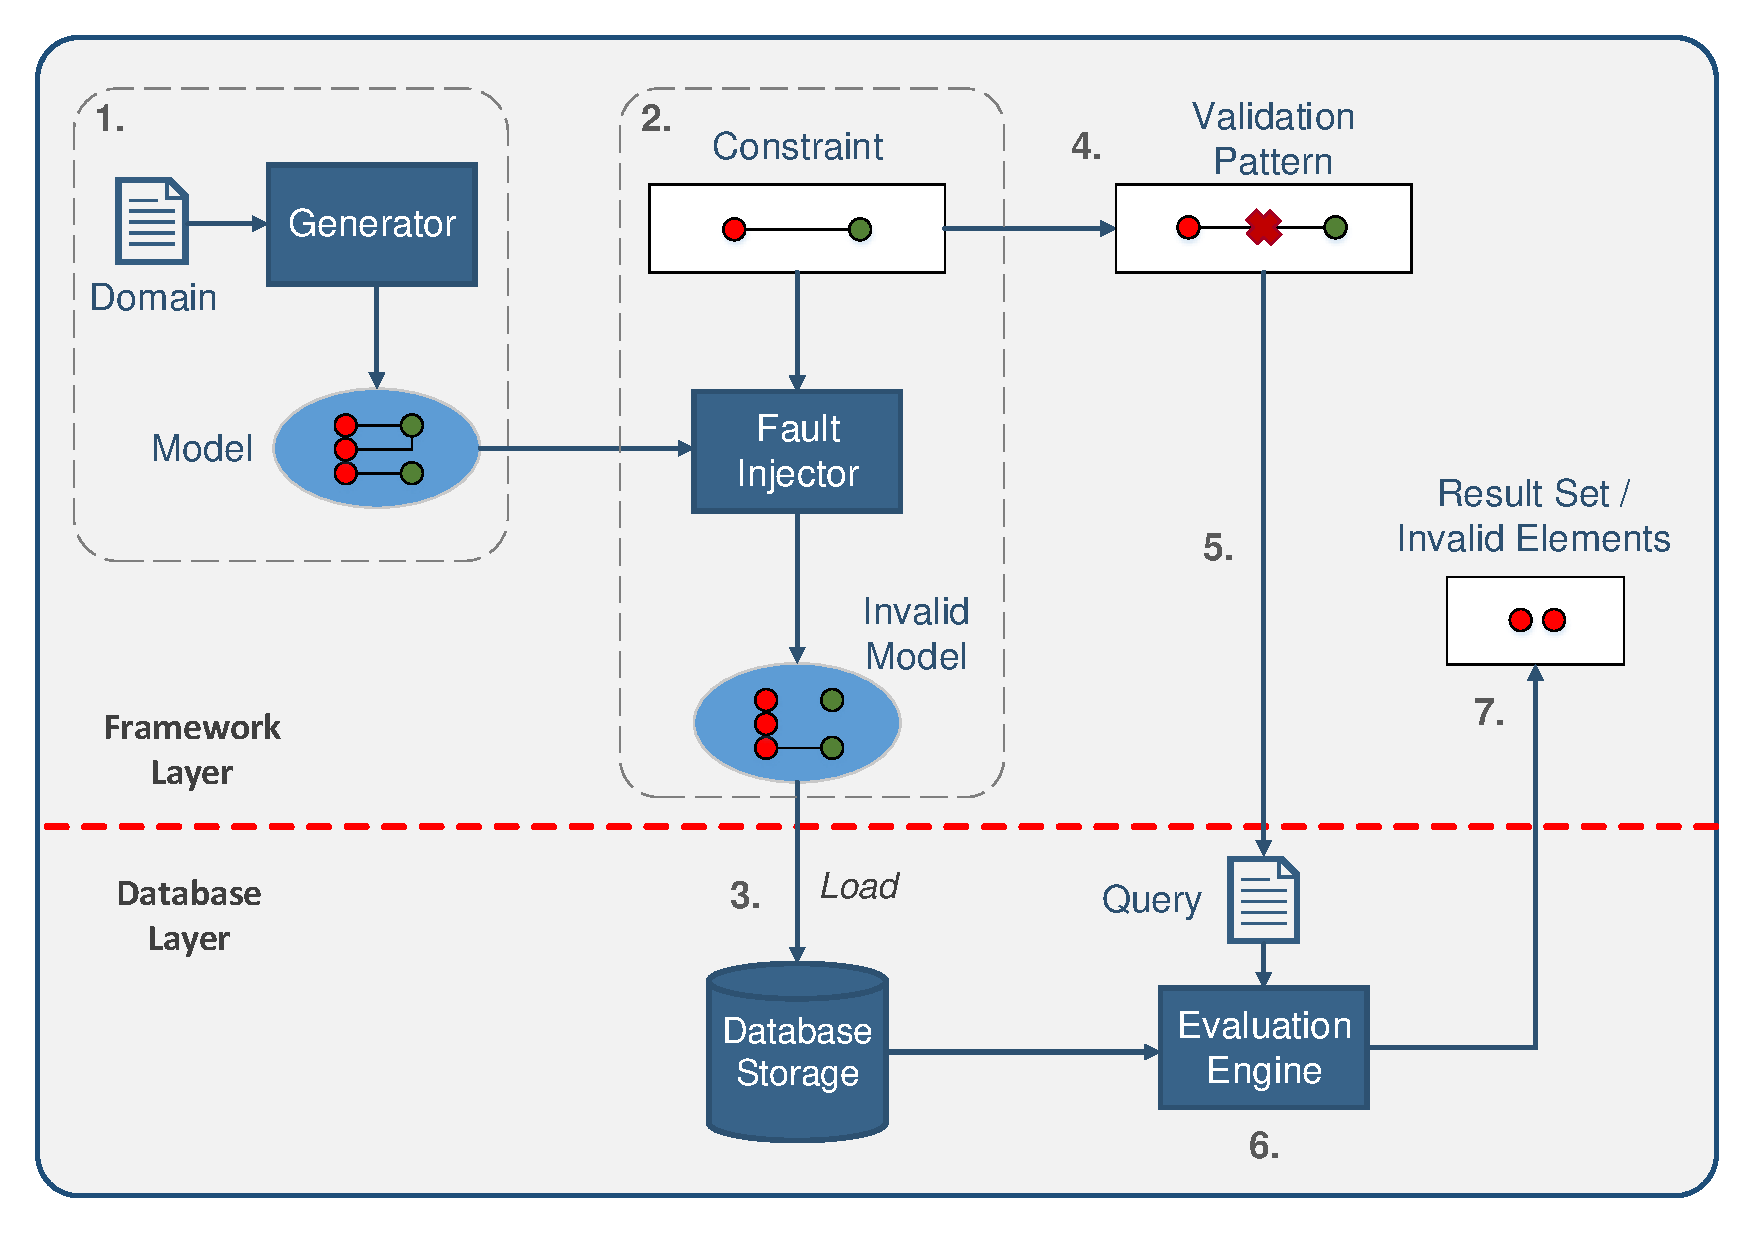
\includegraphics[width=150mm, keepaspectratio]{figures/functionality.pdf}
	\caption{An overview of Train Benchmark.}
	\label{fig:overview_train}
\end{figure}

\begin{figure}[!ht]
	\centering
	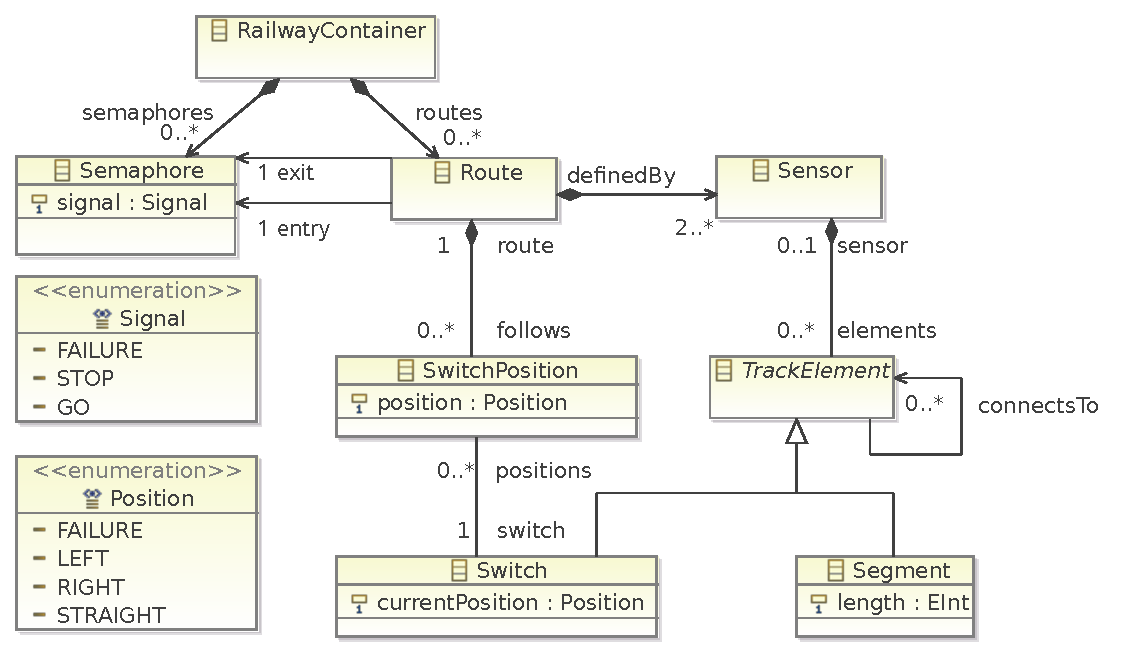
\includegraphics[width=150mm, keepaspectratio]{figures/railway-containments.pdf}
	\caption{The Railway domain of Train Benchmark.}
	\label{fig:tb_domain}
\end{figure}

\subsection{Model Generation}

The Train Benchmark framework uses artificially generated graph-based models for the measurements over a \textit{railway} domain, illustrated in Figure \ref{fig:tb_domain}. In the models, a train route is defined by a sequence of sensors, and the sensors are associated with track elements which are either segments or switches. A route follows certain switch positions which describe the required state of a switch belonging to the route. Each route has a semaphore on its entry and exit~\cite{train_ttc}.

The generated models over the Railway domain are not related to a real-life model, which leads to the fact that the cardinalities of the elements and their distributions do not follow a real model's characteristic, therefore, the measurement results of different databases cannot be claimed to be representative in a real-life use case.

\subsection{Metric-Based Analysis}

The Train Benchmark framework was extended with metric-based analysis in ~\cite{metric_ase}.


\section{Conclusion} \label{sec:benchmark_conclusions}

The represented benchmark frameworks propose different comprehensive use cases to assess the performance of graph queries typically over RDF data. BSBM and DBpedia use representative queries for the measurements that demonstrate real-life use cases, and the SP$^2$Bench framework concentrates on the creation of various systematic queries that investigate the specific RDF data management approaches. The Train Benchmark framework aims a different aspect of performance by concentrating on model validations via graph queries. As a conclusion, these frameworks guarantee a comprehensive performance evaluation of a workload---the model, query and tool---by emphasizing the impact of \textit{queries} to the performance.

However, in case of an arbitrary workload, the \textit{model} also represents a dominating factor to the performance. DBpedia or the SP$^2$Bench framework do not consider model modifications in their workloads, so they do not investigate the impact of various model characteristics to the performance, they only generate the same structural model in different sizes to measure scalability. BSBM proposes update operations on the models, still, it does not investigate model and performance correlations. Even though Train Benchmark considers model transformations, yet, it modifies only one type of element that impacts the result set of the query evaluation, and the generated models are still considered as static models. As a conclusion, all of the introduced frameworks concentrate on the generation of one static model without altering its internal structure and analyzing their influence to the performance.

In order to introduce a new approach to the field of graph-based benchmark frameworks, we focus on elaborating a framework that proposes various models with different characteristics and investigates the relationships between the performance and the internal structure of the model.

The main features of the introduced frameworks and our new approach are summarized in Table \ref{tab:framework_features}.
\begin{table}[ht]
	\footnotesize
	\centering
	\begin{tabular}{l c c c c c}
		\toprule
		Feature & BSBM & DBpedia & SP$^2$Bench & Train Benchmark & Our Approach\\ \hline
		\midrule
		Based on a real-life model &  & \textbullet & \textbullet & &  \\ \hline
		Realistic domain-based queries & \textbullet & \textbullet &  &  & \\ \hline
		Systematic queries  & &  & \textbullet & & \\ \hline
		Model updates & \textbullet &  &  & \textbullet & \\ \hline
		Various models &  &  &  & & \textbullet \\ \hline
		Measurement of scalability  & \textbullet & \textbullet & \textbullet & \textbullet & \textbullet\\ \hline
		Performance metrics  & \textbullet & \textbullet & \textbullet & &  \\ \hline
		Model metrics &  &  &  & & \textbullet \\ \hline
		Various representation formats & &  &  & \textbullet & \\ \hline
		\bottomrule
	\end{tabular}
	\caption{A comparison of existing benchmark frameworks and our approach.}
	\label{tab:framework_features}
\end{table}

Basically, we concentrate on the generation of various models with different internal networks, and we analyze the models and their impact to performance of query evaluations.
	\chapter{Design}

\section{Overview of the Approach}

In this section, we introduce the main notions about our work to analyze model and performance relationships.

Our concept includes the following systems illustrated in Figure \ref{fig:frameworks}. We rely on two existing frameworks in our work: the Train Benchmark and MONDO-SAM frameworks. Furthermore, we the elaborate \framework (MONDO-Metrics-Based Analysis of Performance) and the Homogeneous Graphs Benchmark.
%todo mondo sam cite
\begin{figure}[!ht]
	\centering
	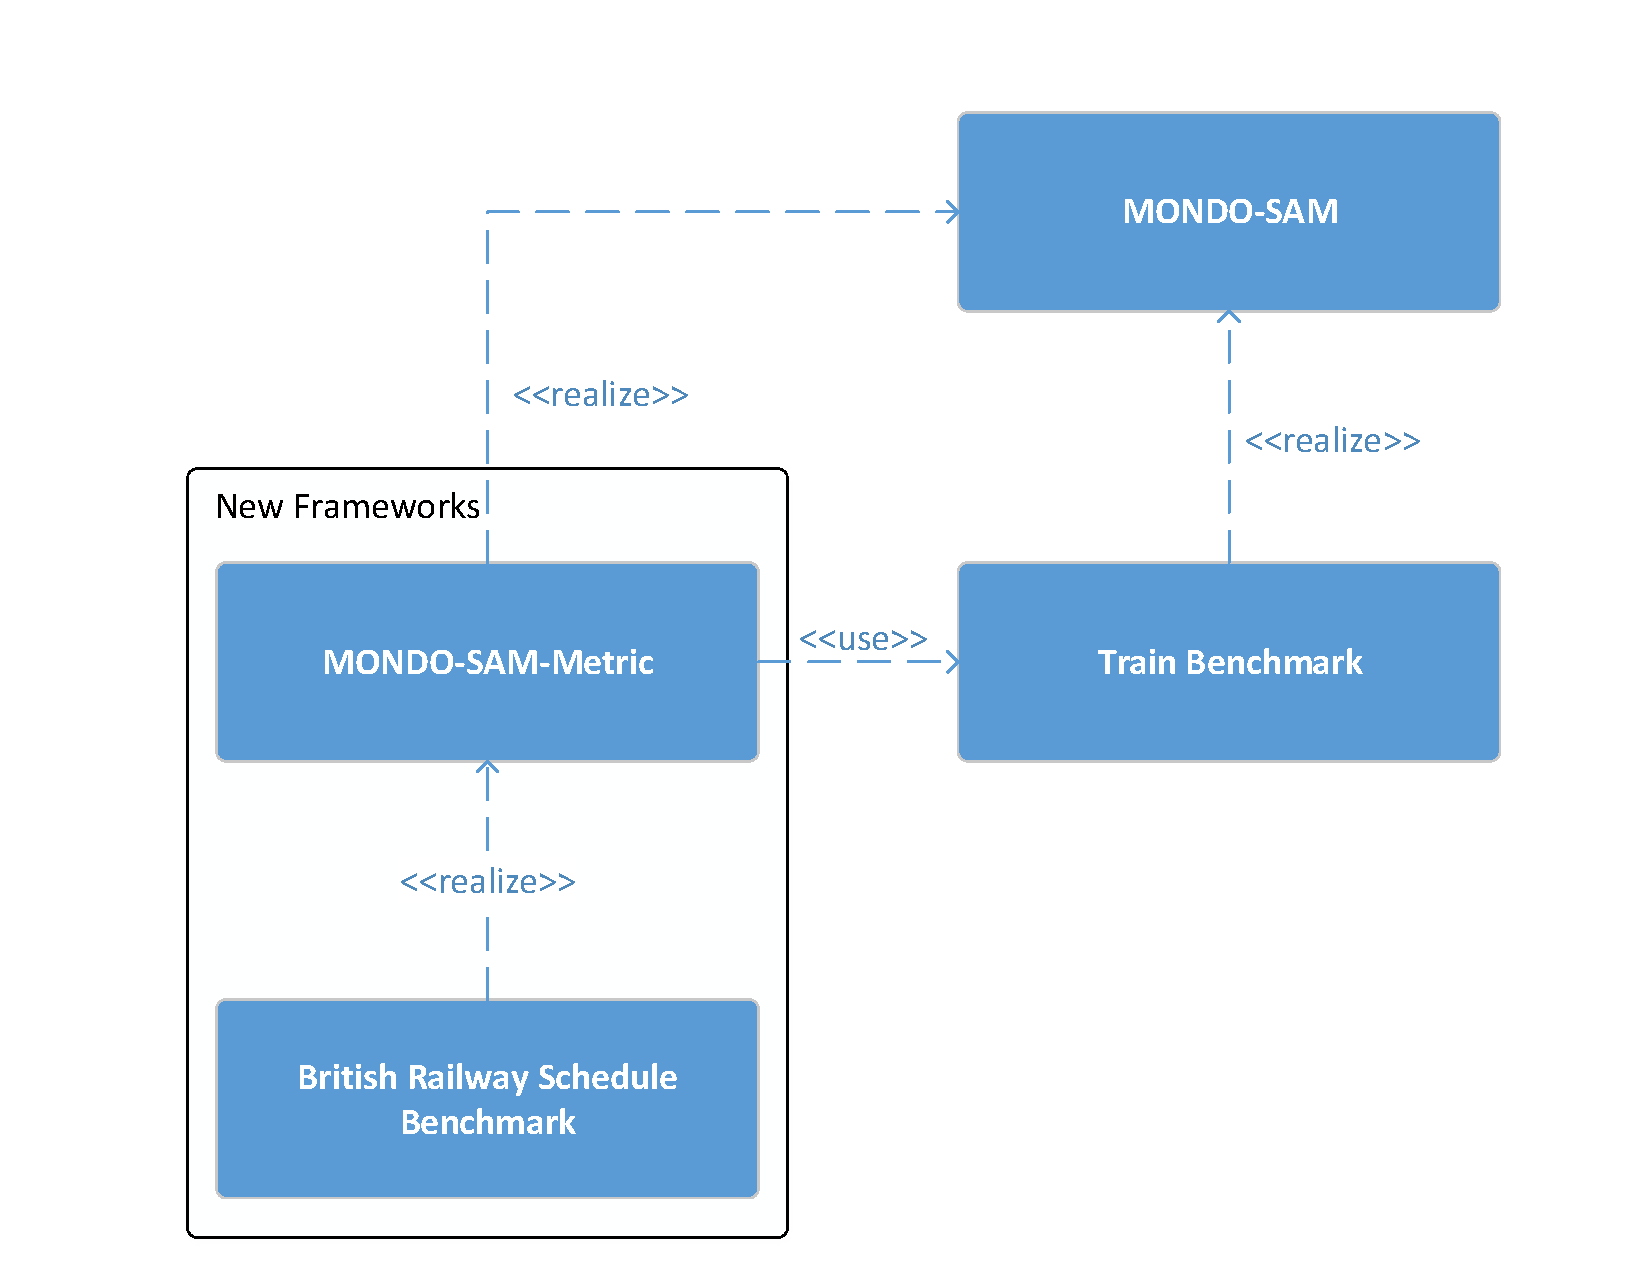
\includegraphics[width=130mm, keepaspectratio]{figures/frameworks.pdf}
	\caption{An overview of the frameworks in our approach.}
	\label{fig:frameworks}
\end{figure}

\paragraph{MONDO-SAM}
The MONDO-SAM framework was created under the project MONDO (Scalable Modeling and Model Management on the Cloud)~\cite{mondo} with the motivation of providing a common benchmark framework in Model Driven Engineering (MDE) for benchmark developers~\cite{mondo-sam}. \sam can be considered as an abstract layer that proposes an evaluation engine to execute arbitrary workflows independently on the current workload. Furthermore, \sam also provides tools for serializing and visualizing the benchmark results.

\paragraph{Train Benchmark}
The Train Benchmark framework is based on the evaluation engine provided by \sam, and it proposes a benchmark for measuring continuous model validations and transformations. The Train Benchmark is presented in detail in Section \ref{sec:train}.

\paragraph{\framework}
The goal of the \map framework is to support model-based performance analysis. To achieve this, it extends \sam with additional features, as it provides a framework for analyzing model and performance relationships in the light of an arbitrary workload by characterizing the performance quantitatively with model related metrics. Similarly to \sam, \map is an abstract framework and can be extended by an arbitrary benchmark case.

\paragraph{Homogeneous Graphs Benchmark}

\begin{figure}[!ht]
	\centering
	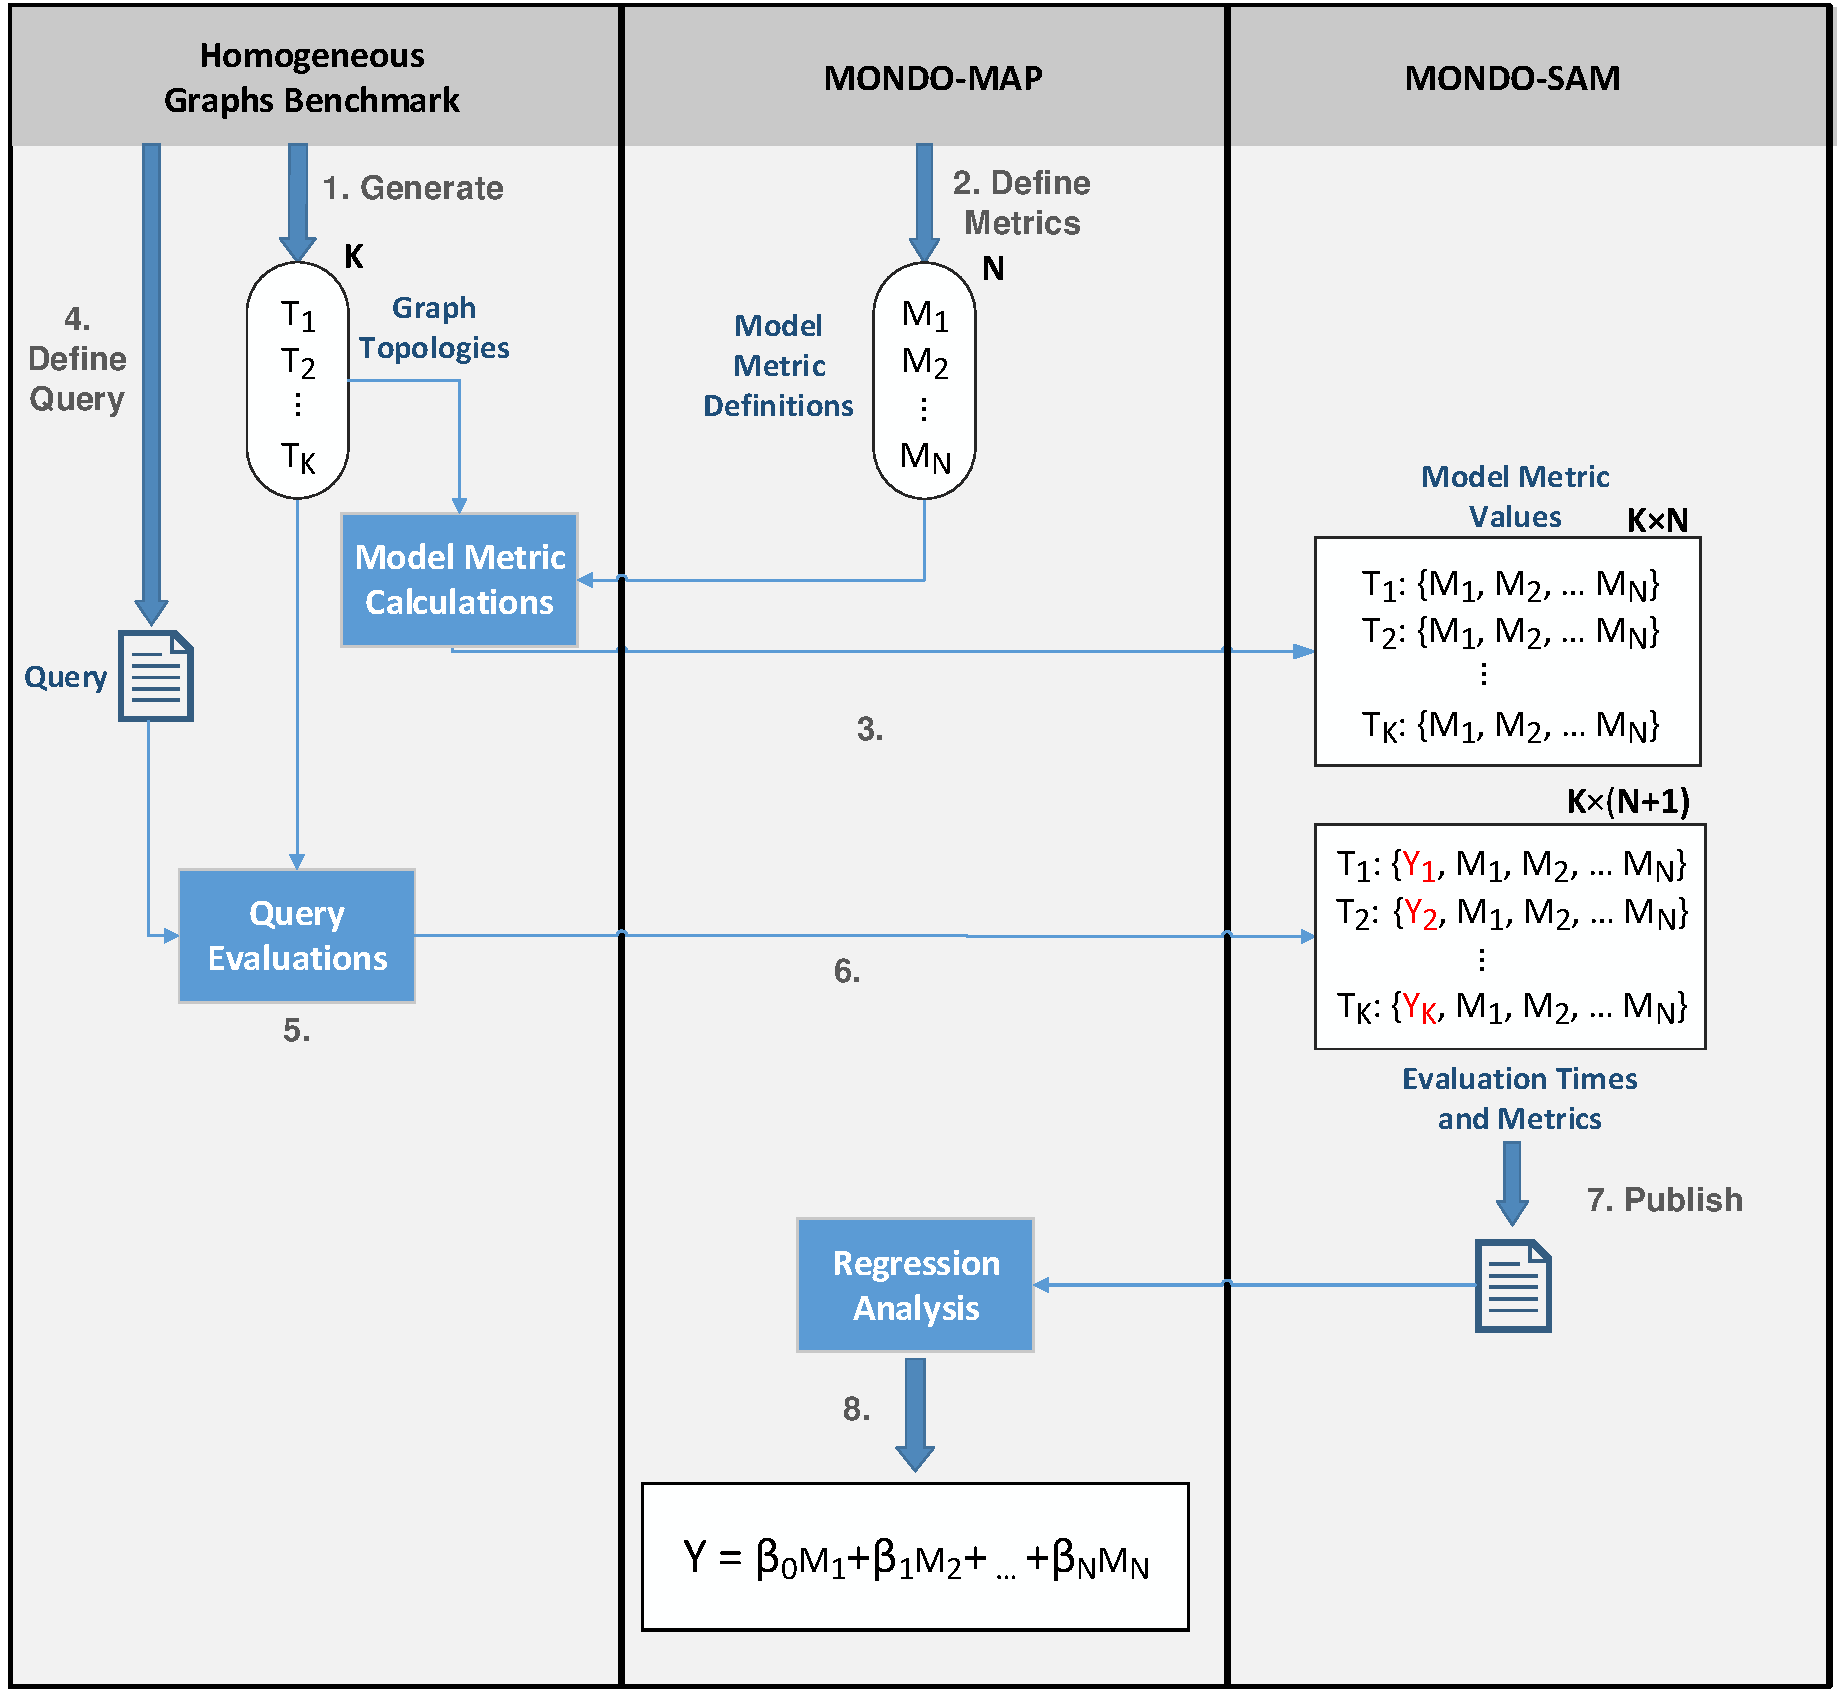
\includegraphics[width=140mm, keepaspectratio]{figures/approach.pdf}
	\caption{The main concept of the metric-based performance analysis.}
	\label{fig:approach}
\end{figure}

The Homogeneous Graphs Benchmark (HG Benchmark) extends the \map framework with a benchmark case for RDF databases. It generates homogeneous graphs---well-known network topologies---and it investigates the relationships between the model metrics and performance of query evaluations with respect to an arbitrary query and tool. The goal is to generate artificial graphs with various characteristics and obtain a spread in their descriptive metrics, and thus showing a quantitative connection between model metrics and performance. As Figure \ref{fig:frameworks} suggests, in the HG Benchmark we use a part of the components of the Train Benchmark that are adequate for our purpose as well.

Figure \ref{fig:approach} illustrates the main concept of our work. First, the HG Benchmark generates different $K$ graph topologies. Using the graph metric definitions from \map (2.), we calculate the descriptive metrics for every topology in step 3. In the next two steps (4-5.) we define a query and evaluate it on every topology in the system under benchmark. The measurement result is the query evaluation time ($Y$) that represents another variable belonging to the topologies besides their metrics (6.). As it was mentioned before, the \sam framework is responsible for publishing the benchmark results (7.). Finally, in \map we analyze the results by creating regression models to estimate the influence of metrics to the performance.

%\subsubsection{Challenges}

%Three challenges can be found in our research. At first, we have to provide a solution in the HG benchmark to generate models with different %characteristics that impact the performance of a particular query and cause a deviation in evaluation time. 
%Second, we have to find model metrics that are able to characterize the models individually. Furthermore, these attributes must be suitable to %create quantitative relationships among them and the evaluation times.

\section{Models and Metrics}
\subsection{Real-Life Networks}

%todo copy heavy tail to background
In the field of graph theory, the internal structures of real-life networks are comprehensively investigated. The main approach in the analysis of these networks is to explore the degree distributions and study the specific metrics---typically the clustering coefficients, average degrees, average shortest paths---that are suited to characterize the graphs appropriately. Based on the degree distributions and metrics, one can draw a conclusion how a particular real-life network shows a similar characteristic to the well-known topologies such as the random graph, scale-free model, small-world model of Watts-Strogatz or the hierarchical network.\\
For example, the network of World-Wide-Web is studied in~\cite{www1} and~\cite{www2} as well, and the authors observe that the degree distribution of the \textit{www} follows a power-law distribution with a heavy tail, which indicates the presence of web pages with significantly higher degrees than the average degree. Since the probability of occurrences of these web pages is considerably low, the connectivity of the world-wide-web can be represented by the scale-free model of Barabási and Albert.

More examples can be found in the study of Barabási and Albert~\cite{statistical_mechanics}, as they review the advances of different publications and investigate the characteristics of different real-life networks. Empirical results prove that the \textit{movie actor collaboration network}, \textit{cellular networks}, \textit{phone call} and \textit{citation} networks also follow power-law distributions. Many of the studied networks can be considered as scale-free models, however, a part of these graphs---for example the network of movie actors---also show small-world properties and a high clustering coefficient in their connectivity similarly to the Watts-Strogatz or hierarchical topology.

As far as the Watts-Strogatz model---and the random graph---are concerned, their specific degree distribution---Poisson---rarely appears in the real-life networks, as it is emphasized in~\cite{random_study}. However, the small-world property of the WS models frequently appears in the real-life networks. In practice, none of the artificial topologies can be identified perfectly to real-life models, however, the representative metrics of these artificial networks can be observed in real-life networks as well. 

We assume that those metrics that show high deviations among the different topologies are suited to characterize and identify them individually, furthermore, they may able to characterize an arbitrary graph as well. If these metrics are capable to characterize entirely different networks, then we assume that these metrics are the key to characterize the performance of query evaluations.

\subsection{Network Topologies and Representative Metrics} \label{sec:topology_metric}

Barabási and Albert inspect the natures of the well-known graph topologies in~\cite{statistical_mechanics}, such as the random graph, scale-free and the Watts-Strogatz model. As a main result, they observe that there are significant differences among the topologies regarding specific graph metrics. Based on their study and the research of hierarchical graphs~\cite{hierarchical}, the following metric deviations are assumed between the four topologies, illustrated in Table \ref{tab:topology_metrics}. The random graph is considered as a reference point, and every value is compared to its metrics by assuming that the networks are in the same size.
\begin{table}[ht]
	\footnotesize
	\centering
	\begin{tabular}{ l c c c c}
		\toprule
		Metric & Random & Hierarchical & Scale-free & Watts-Strogatz \\ 
		\midrule 
		\textbf{Max Degree} & $\bullet$ & $\bullet$$\bullet$$\bullet$ & $\bullet$$\bullet$$\bullet$ & $\bullet$ \\ \hline
		\textbf{Clustering Coefficient} & $\bullet$ & $\bullet$$\bullet$$\bullet$ & $\bullet$ & $\bullet$$\bullet $\\ \hline
		\textbf{Avg Shortest Path Length} & $\bullet$ & $\bullet$$\bullet$ & $\bullet$ & $\bullet$$\bullet$ \\ \hline
		\bottomrule
	\end{tabular}
	\caption{Graph topologies and their descriptive metrics}
	\label{tab:topology_metrics}
\end{table}
%todo describe bullets in detail
As Table \ref{tab:topology_metrics} demonstrates, each topology can be characterized by different metric values, which leads to the assumption that if the diversity between the topologies may cause high variance in the performance of a particular query evaluation, then these metrics are adequate to characterize the model and performance relationships quantitatively.

%todo use lattice ref in background
%todo emphasize lattice, random and p value in background, maybe add a picture as well

However, the values of metrics in Table \ref{tab:topology_metrics} are misleading due to the reason that the metrics of the Watt-Strogatz model highly depend on the initialization of the network, namely, the value of $p$ probability that is used in the generation.

\begin{figure}[!ht]
	\centering
	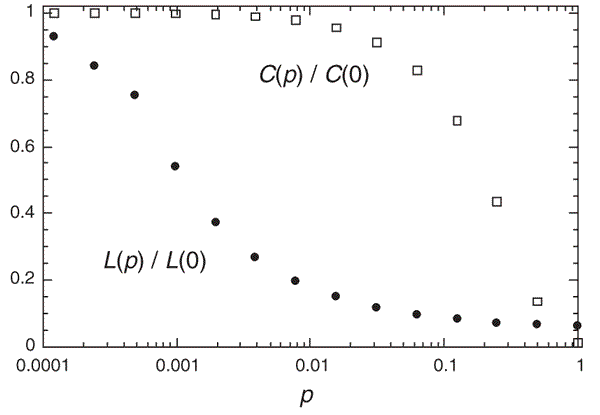
\includegraphics[width=100mm, keepaspectratio]{figures/ws_metrics.png}
	\caption{Characteristic path length $L(p)$ and clustering coefficient $C(p)$ of Watts-Strogatz model~\cite{ws_metrics}}
	\label{fig:ws}
\end{figure}

By modifying $p$, the Watts-Strogatz model represents a bridge between a lattice and a random graph. As Figure \ref{fig:ws} illustrates, the clustering coefficient $C(p)$ and the average shortest path ($L(p)$) metrics are changed with respect to $p$ scaling. The values are normalized by $L(0)$ and $C(0)$ that represent the clustering coefficient and average shortest path metrics for a lattice graph. As a conclusion, the Watts-Strogatz model shows significant deviations in these two metrics in the light of the $p$ probability value. 

%todo add betweenness reference to background
Besides the models in Table \ref{tab:topology_metrics}, the metrics also require modifications. The problem is that the maximum degree metric alone does not include a comprehensive information about the internal structure of the network, since it does not emphasize the role of a node with maximum degree in the connectivity of the graph. Hence, we use another metric---the \textit{betweenness centrality}---which characterizes adequately the importance of a higher degree, since the higher value of betweenness centrality belongs to a vertex, the more shortest paths include that node, symbolizing that node represents the center in the graph.

After these modifications, the topologies and the related metrics are shown in Table \ref{tab:topology_metrics2}. WS-$p$ indicates the Watts-Strogatz model with a probability value of $p$. The values of the betweenness centrality are determined by our initial assumption considering that the \textit{center} node in a hierarchical network and the \textit{hubs} in a scale-free model may occur more times in the shortest paths due to the fact that they have higher degrees. The main conclusion is that we can achieve a higher deviation among the metric values by using these topologies, and thus, in the following we concentrate on these networks.
\begin{table}[ht]
	\footnotesize
	\centering
	
	\begin{tabular}{ l c c c c c c}
		\toprule
		Metric & Random & Hierarchical & Scale-free & WS-0.1 & WS-0.01 & WS-0.001 \\ 
		\midrule 
		\textbf{Max Degree} & $\bullet$ & $\bullet$$\bullet$$\bullet$ & $\bullet$$\bullet$$\bullet$ & $\bullet$ & $\bullet$ & $\bullet$ \\ \hline
		\textbf{Clustering Coefficient} & $\bullet$ & $\bullet$$\bullet$$\bullet$ & $\bullet$ & $\bullet$$\bullet$ & $\bullet$$\bullet \bullet$ & $\bullet$$\bullet$$\bullet$\\ \hline
		\textbf{Avg Shortest Path Length} & $\bullet$ & $\bullet$$\bullet$ & $\bullet$ & $\bullet $ & $\bullet \bullet$ & $\bullet$$\bullet$$\bullet$\\ \hline
		\textbf{Betweenness Centrality} & $\bullet$ & $\bullet$$\bullet$$\bullet$ & $\bullet$$\bullet$ & $\bullet$ & $\bullet$ & $\bullet$\\ \hline
		\bottomrule
	\end{tabular}
	\caption{Graph topologies and their descriptive metrics with extensions}
	\label{tab:topology_metrics2}
\end{table}

\section{Metric and Performance Comparison}

Showing performance and metric relationship is an essential goal of our approach. The first notion is the search of correlations between the metrics and performance.

A similar problem is studied in~\cite{algebraic1} and~\cite{algebraic2}, where the authors generate well-known topologies and inspect the connectivity and robustness of the networks. In their case, a network is said to be robust if its performance is not sensitive to the changes in topology. In~\cite{algebraic1}, the \emph{algebraic connectivity} (not discussed in detail in this report) metric is studied to search robustness and metric relationships, however, they show that the algebraic connectivity is not trivially correlated to the robustness of the network.

The authors in~\cite{algebraic2} investigate the impact of betweenness centrality, algebraic connectivity and average degree to robustness, and they also draw the conclusion that there is no unique graph metric to satisfy both connectivity and robustness objectives while keeping a reasonable complexity, since each metric captures some attributes of the graph.

Partly based on the advances of these two publications and our initial assumption of the topologies and their metrics (Table \ref{tab:topology_metrics2}), we expect that we cannot find a correlation between one metric and the performance, hence, we suspect that only the ensemble of more metrics is suited to find relationship.

In order to find quantitative connections, we use regression analysis to show how the various metrics impact the performance. 

\subsection{Choosing the Sample}

By using regression analysis on a sample, it is important to regard the sample to be unbiased. In our case, a bias in a sample of graph topologies means a variation in the size of the models. Obviously, one topology in the sample with larger amount of nodes can bias the connection between the models and the performance, therefore, our framework must support the generation of \textit{uniform} models\footnote{From now on, under the concept of uniform models we mean models with approximately equal number of nodes and edges, despite the diversity of their internal structures.} with respect to the amount of nodes and edges, even in the case of different topologies.

	\chapter{Contributions}

In the following sections, we present the main contributions related to the \framework~framework and the Homogeneous Graphs Benchmark.

\section{Overall Architecture}

Figure \ref{fig:architecture} depicts the frameworks and the main components belonging to them, additionally, it also denotes which components are reused from Train Benchmark.

\begin{figure}[!ht]
	\centering
	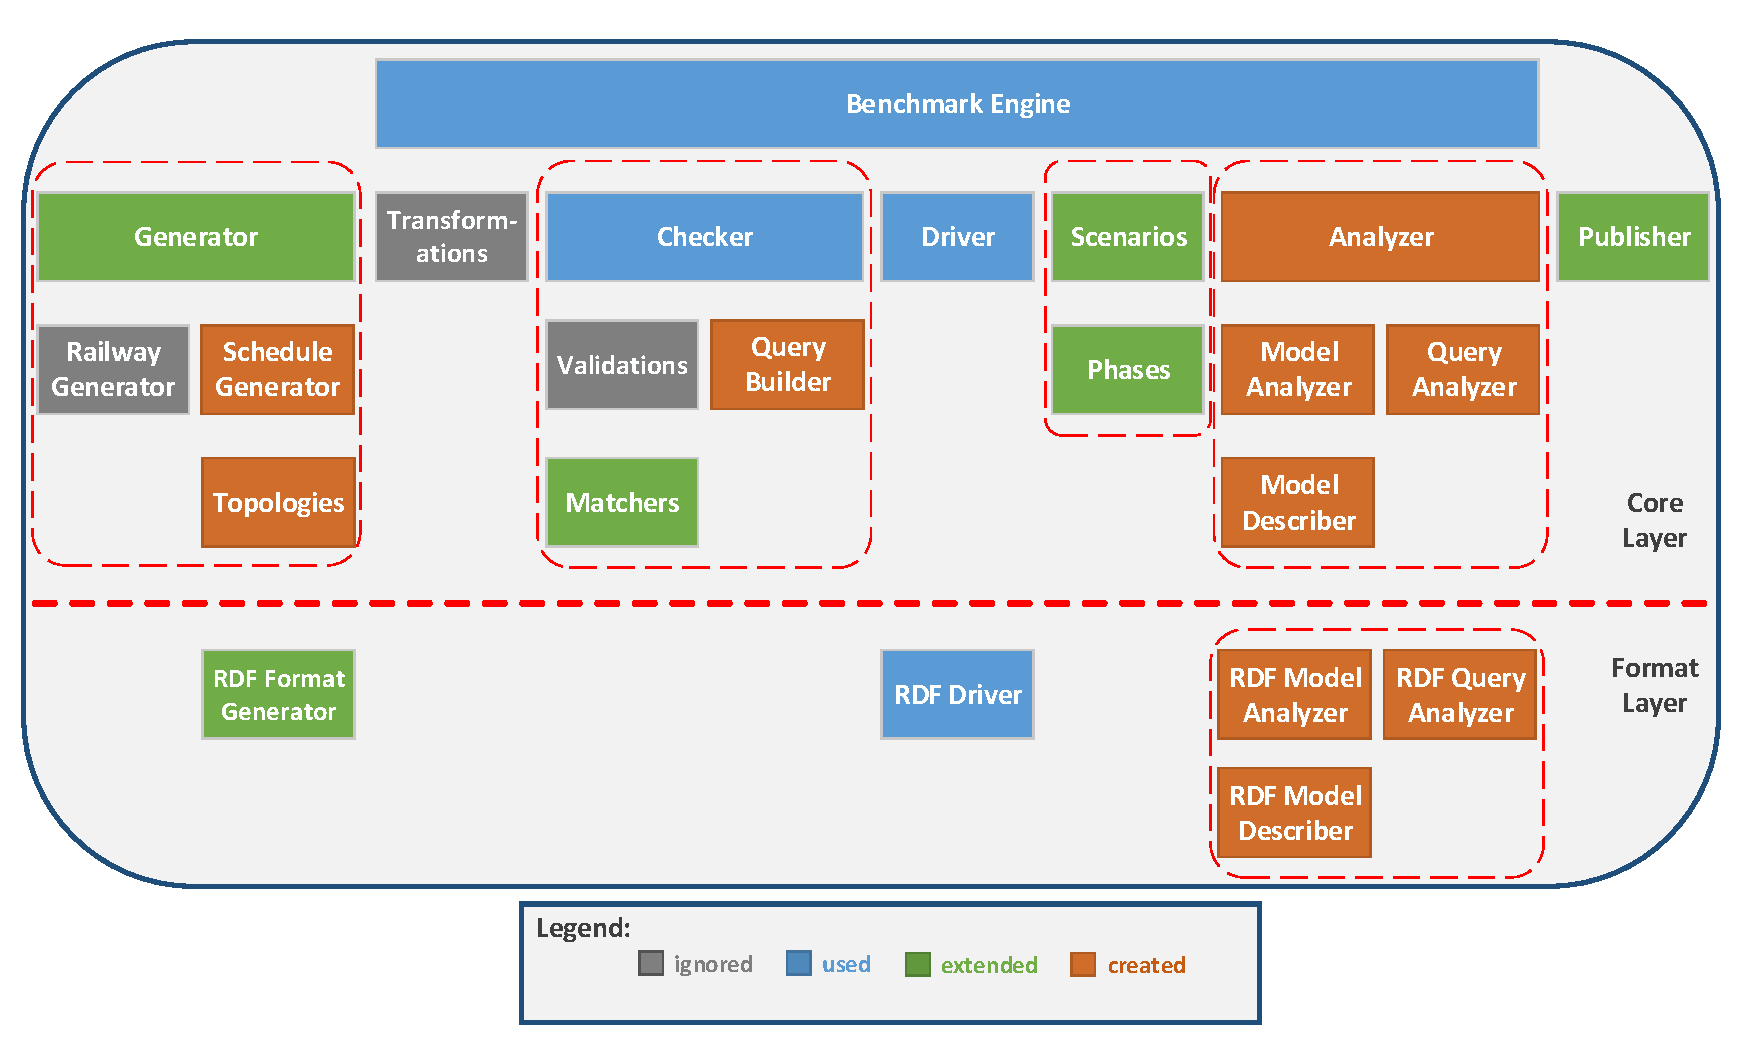
\includegraphics[width=150mm, keepaspectratio]{figures/architecture.pdf}
	\caption{The architecture of our approach.}
	\label{fig:architecture}
\end{figure}

In the following, we introduce the components.

\paragraph{Benchmark Engine}
The \textsf{Benchmark Engine} in MONDO-SAM is responsible for evaluating an arbitrary sequence of phases consecutively. A phase is considered as the atomic execution unit in a benchmark. The engine also measures the evaluation times of phases, hence, it is the component that measures the performance of query evaluations in our work.

\paragraph{Analyzer Components}

The \textsf{Model} and \textsf{Query Analyzer} units belong to the \framework~framework and define an interface for the metrics calculation. The \textsf{Model Analyzer} investigates the model related metrics, and the \textsf{Query Analyzer} relates to the query definitions. As it can be observed, the concrete metric calculations---\textsf{RDF Model Analyzer} and \textsf{RDF Query Analyzer}---appear in the HG Benchmark.

\paragraph{Metrics}

The definitions of metrics---such as \textsf{Model Metrics}  and \textsf{Query Metrics}---can be found in \framework. The model metrics symbolize graph metrics with applying the commonly used naming conventions from graph theory. Note that the HG Benchmark does not contain further RDF-based metrics implying that we use the graph-based naming conventions in our work.\\
The query metrics describe the complexity of a query itself, without considering its performance in a particular setting.

\paragraph{Generators}

The generator components belong to the HG Benchmark. The abstract \textsf{Generator} unit is utilized from Train Benchmark. The \textsf{Stations Generator} component is responsible for transforming the real-life British Railway Stations model to RDF. Last, the \textsf{Topology Generators} construct different homogeneous graphs fitting to well-known topologies and transform them to RDF format.

\paragraph{RDF Driver}
The \textsf{RDF Driver} manages the connections between the measured RDF databases and the benchmark framework, furthermore, it also accomplishes the loading of the models. 

\paragraph{Query Executor and Query Builder}

The query evaluations are initiated by the \textsf{Query Executor} component. The \textsf{Query Builder} is responsible for creating and altering the query definitions in runtime.

\section{British Railway Stations}

In order to test our regression models on an entirely different graph, we introduce a real-life model to our work. We use a model of train stations provided by the \textit{Network Rail} company that runs, maintains, and develops Britain's rail tracks~\cite{network_rail}. Network Rail publishes a number of different data available to developers, one of them is a \textit{daily extracts and updates of train schedules}~\cite{schedules_data} that which formed the basis of our data set.

The data contains approximately 10~000 British stations that belong to train schedules as destinations. We concentrate on the network of stations, and map it to a graph where every vertex symbolizes a station. An edge is drawn between two nodes---\ie two stations---if these stations appear consecutively in a destinations path belonging to a schedule.

\section{Uniform Model Generation}

It is an essential requirement of the HG Benchmark to guarantee uniform model generation among the topologies indicating the same size of the generated models. We propose a model generation technique to generate topologies with the same amount of nodes and edges.

\subsection{Number of Nodes}

The random graph and the Watts-Strogatz model are constructed by initializing $|V| = N$ number of vertices, and then the algorithms determine which one of them become adjacent. In the scale-free model generator, the nodes are created incrementally until $|V| = N$, and a precise number of nodes can be obtained regarding these topologies.

The only problem about generating topologies with a certain number of nodes is the recursive algorithm of the hierarchical graph, which algorithm has to be terminated.

\subsubsection{Termination of the Hierarchical Network Generation Algorithm}\label{sec:hierarcical_contribution}

Since the generation of hierarchical network is recursive instead of being incremental---as in the case of the three other topologies---it is necessary to determine a termination from the recursive algorithm. The termination point is evident, as soon as the number of created nodes reaches the limit, the algorithm has to be stopped. However, it cannot be predicted in which phase the algorithm stops exactly. As a consequence, the possible problems have to be managed.

\begin{figure}[!ht]
	\centering
	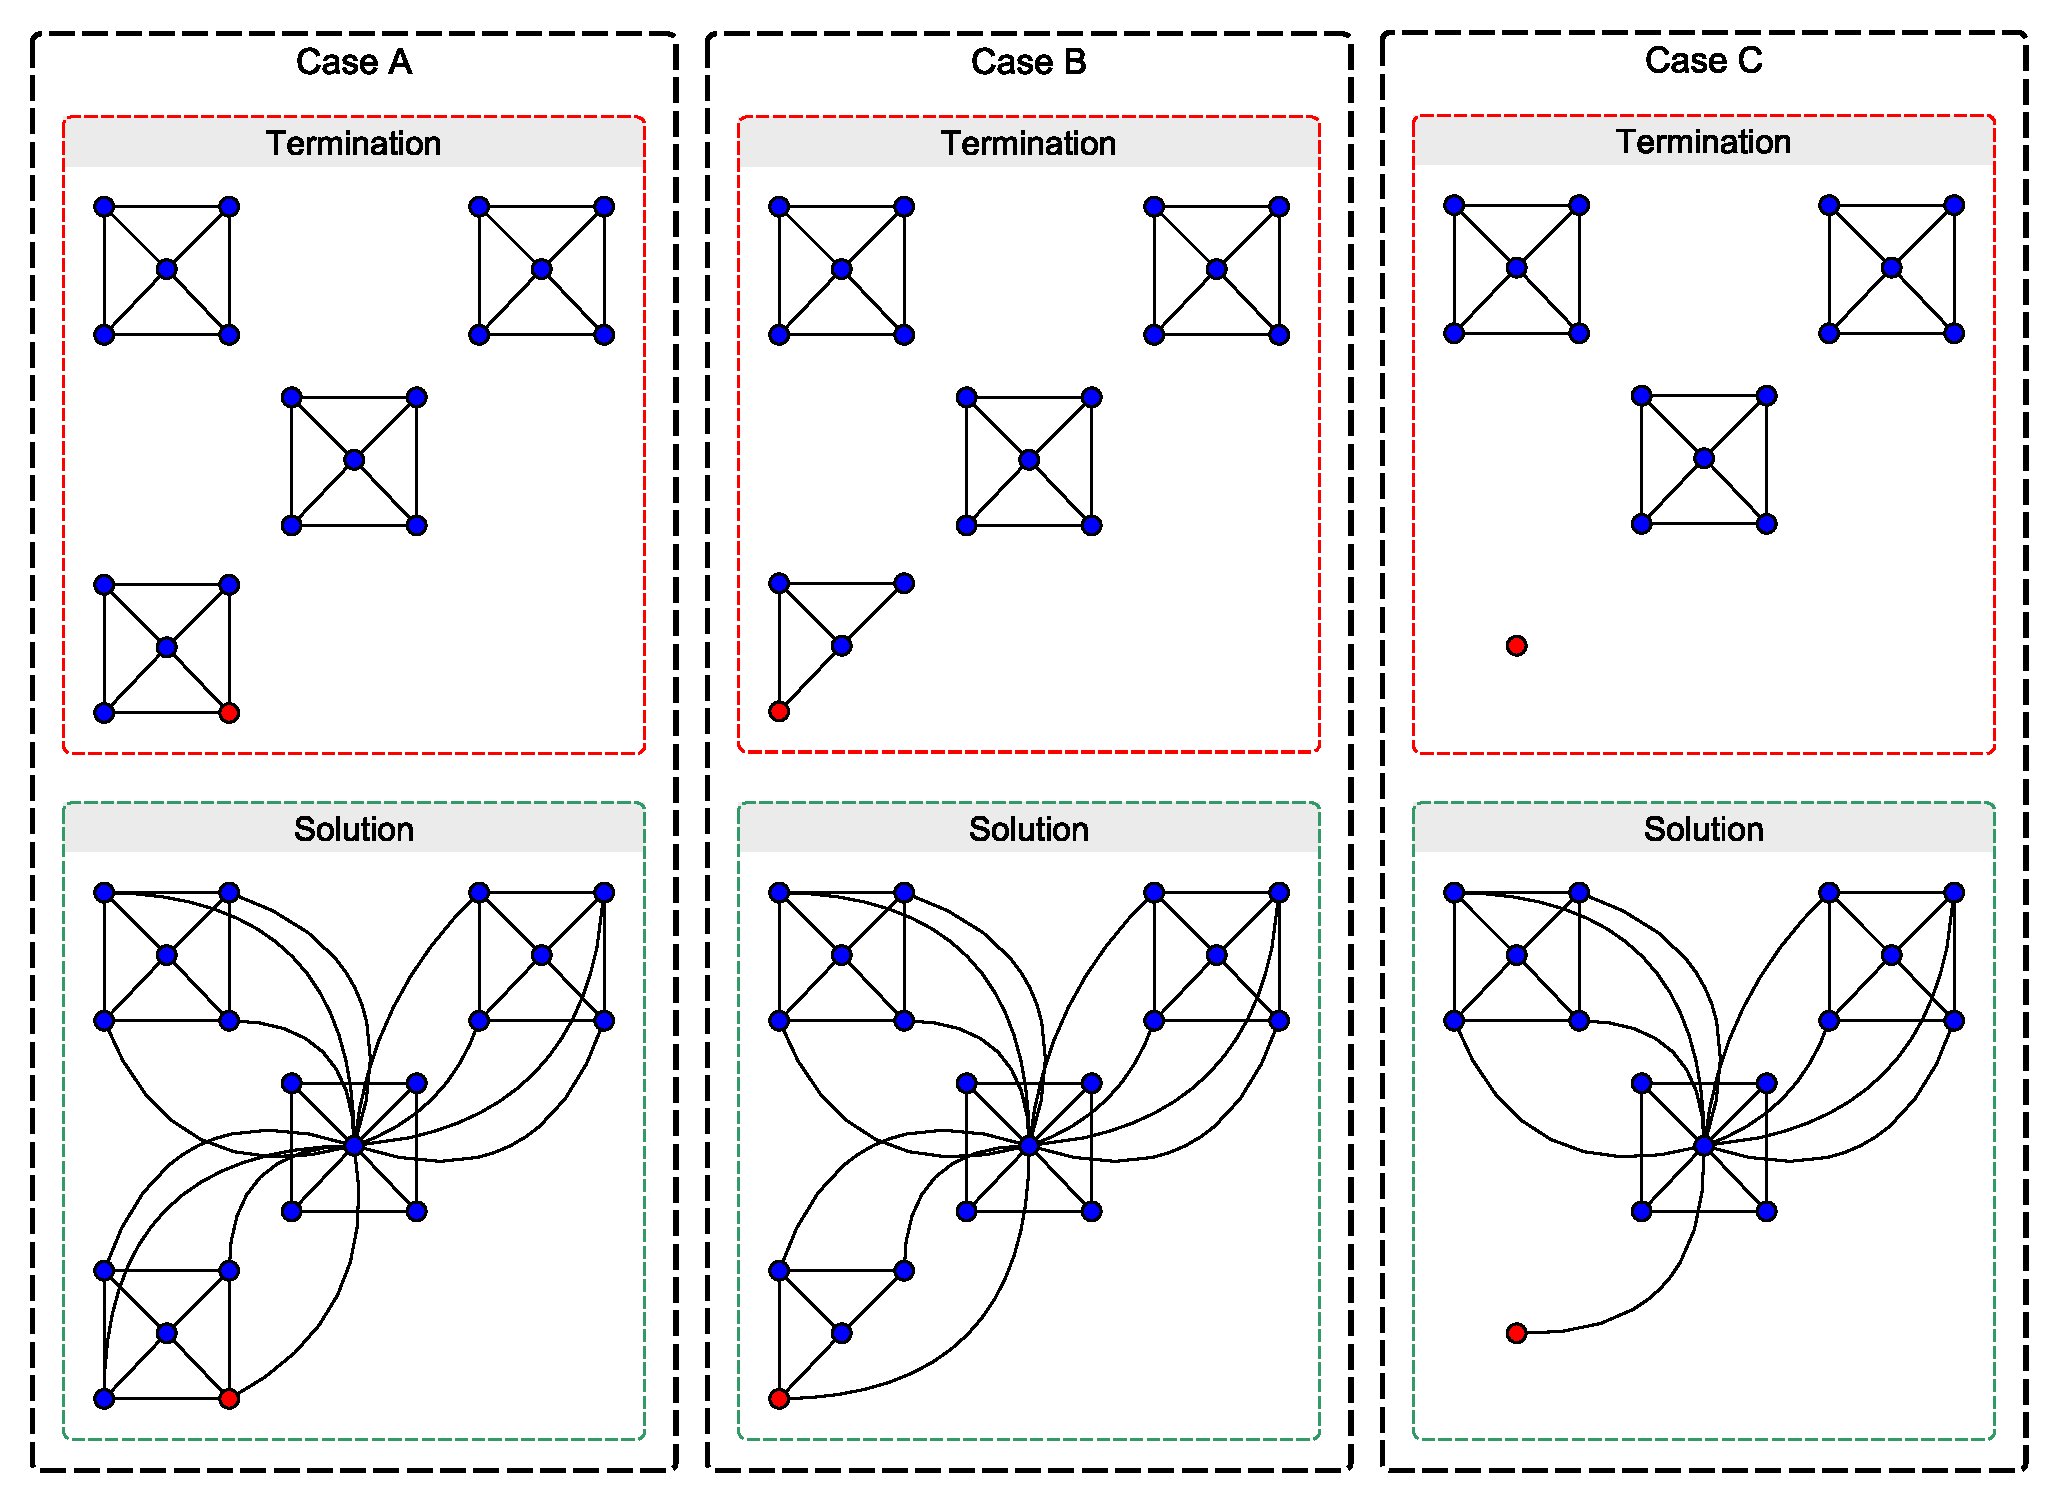
\includegraphics[width=150mm, keepaspectratio]{figures/hierarchical.pdf}
	\caption{Possible termination problems in the hierarchical graph generation.}
	\label{fig:hierarchical_problems}
\end{figure}

The possible problematic cases are demonstrated in Figure \ref{fig:hierarchical_problems}. In \textsf{Case A}, \textsf{B}, and \textsf{C}, the expected numbers of nodes are 20, 19, and 16, respectively. As it can be observed in these cases, this limit is always reached before the fourth cloning occurs, since 5 clusters should be created with 25 vertices at the end of this step in the recursion.

In the solution in \textsf{Case A}, the generator stops the cloning procedure and connects the diagonals to the center. Regarding \textsf{B}, the termination happens during the generation of a cluster. As a solution, the last cluster becomes partial, and similarly, every diagonal is attached to the center. \textsf{Case C} represents that scenario when the last cluster only consists of one node. To prevent isolation, the last vertex is considered as a diagonal, and be connected to the center.

\subsection{Number of Edges}

%todo note that the diagonal nodes are also connected — links not visible on hierarchical graph
In terms of the random graph, scale-free, and WS model, their generation algorithms can be adjusted arbitrarily, meaning that an optional number of nodes or edges can be achieved. As a matter of fact, reaching a certain amount of nodes or edges in these networks are handled separately.

Unfortunately, the creation of nodes and edges in the hierarchical graph occur together. Since the amount of edges depends on the number of nodes and iterations in the recursive algorithm, it cannot be configured arbitrarily. A solution is that we adjust the other topologies to have the same number of edges as the hierarchical model. This solution requires to calculate the exact number of edges in a hierarchical network with respect to the iteration.

\subsubsection{Estimating the Number of Edges in Hierarchical Graphs}

The literature relating to hierarchical graphs does not mention the exact number of edges or its correlation to the amount of nodes, hence, we propose a solution to estimate $|E|$ in the recursive algorithm for every iteration.

At first, let us define the necessary variables hereunder:
\begin{itemize}
	\item{$i$}: represents the current iteration in the original hierarchical algorithm.
	\item{$c$}: indicates the number of clones in every iteration.
	\item{$n$}: the cluster size is denoted by $n$, which is a $K_n$ complete graph.
	\item{$F_i$}: indicates the constructed graph after the $i.$ iteration. %todo why F? maybe change it to H later
	\item{$|E_{F_i}|$}: the number of edges of $F_i$.
\end{itemize}

The algorithm works as follows. In the 0.~iteration, the hierarchical graph consists of one $K_n$ cluster. Formally, $F_0 = K_n$, and $|E_{F_0}| = |E_{K_n}| = \frac{n \cdot (n-1)}{2}$. In the 1. iteration, the algorithm clones $F_0$ $c$ times, and connects the peripheral nodes from each $F_0$ to the center node. It entails that 
\begin{align}\label{eq:f1_version1}
	|E_{F_1}| = (c+1) \cdot |E_{K_n}| + c \cdot (n - 1)	
\end{align}
since $c+1$ number of $K_n$ can be found in $F_1$, and $c \cdot (n - 1)$ edges can be drawn from the $c$ number of replicas to the center.

Note that in the first iteration $K_n$ can be substituted with $F_0$, and the algorithm in the first part of the $i.$ iteration creates $c$ replicas of the result of the $i-1.$ iteration, namely, $F_{i-1}$. In the second part of the $i$ iteration, the algorithm connects the clusters from the cloned replicas to the center node. These connections are made between the peripheral nodes in each replica and the center, which indicates that in the $i.$ iteration the algorithm connects $n-1$ peripheral nodes from $c$ number of replicas of $F_{i-1}$. Due to $F_{i-1}$ includes $c^{i-1}$ number of clusters, we obtain

\begin{align}\label{eq:fi_formula}
	|E_{F_i}| = (c+1) \cdot |E_{F_{i-1}}| + c \cdot c^{i-1} \cdot (n - 1)	= (c+1) \cdot |E_{F_{i-1}}| + c^i \cdot (n - 1)
\end{align}

Equation \ref{eq:fi_formula} is equal to the number of edges of a completely finished hierarchical network, however, the generation algorithm in the HG Benchmark is possibly terminated to reach a certain number of nodes which leads to the fact that $|E_{F_i}|$ must be scaled down by the proportion of the maximum ($|V_{F_i}|$) and the required number ($|V_H|$) of vertices. If the hierarchical graph we intend to generate is denoted by $H$, then
\begin{align}\label{eq:h_formula}
	|E_H| = |E_{F_i}| \cdot \frac{|V_H|}{|V_{F_i}|}
\end{align}
where $\frac{|V_H|}{|V_{F_i}|} \leq 1$.

By using Equation \ref{eq:h_formula}, we can calculate the number of edges of a hierarchical graph and configure the other topologies to reach the same quantity.

\subsubsection{Configuring the Random Graph Model}
From the two most well-known algorithms, Gilbert's $G(n,p)$ model is adapted to the framework, which implies that the exact value of $p$ has to be determined from the number of edges in the hierarchical graph, $|E_H|$. Based on~\cite{random_p}, the $p$ probability can be calculated from the number of nodes and edges as follows:
\begin{align}
	p = \frac{|E_H|}{\binom{|V|}{2}}
\end{align}
where $|V|$ denotes the number of nodes.

\subsubsection{Configuring the Watts-Strogatz Model}\label{sec:watts_generation}

Regarding the Watts-Strogatz model, in the beginning of the generation algorithm, $K$ number of consecutive nodes are connected to each other. During the algorithm, by rewiring the edges the amount of $|E|$ is not changed. As a conclusion, in order to achieve a uniform size similarly to the hierarchical graph, $K$ has to be adjusted as $K = \frac{|E_H|}{|V|}$.

Generally, the $K$ value in the algorithm is a constant integer. In order to configure the WS model properly, we extend the algorithm by defining an inclusive lower bound ($K_1$) and upper bound ($K_2$) for $K$, as $K\in[K_1, K_2]$. We also assign a $p$ probability to $K$ that determines the likelihood that $K$ is equal to $K_2$ and $1-p$ to $K_1$. Derived from the equation $K = \frac{|E_H|}{|V|}$, it results in $K_1 = \Big\lfloor\frac{|E_H|}{|V|}\Big\rfloor$ and $K_2 = \Big\lceil\frac{|E_H|}{|V|}\Big\rceil$, additionally, the $p$ probability equals to the fractional part, as $p = \Big\{\frac{|E_H|}{|V|}\Big\}$. Hence, by turning $K$ to a random variable, we can generate WS models with the same number of edges as $|E_H|$.

\subsubsection{Configuring the Scale-Free Model}

The scale-free topology is generated incrementally, since every step a new node is inserted to the graph with $m$ new connections. To obtain $|E_H|$ edges, the $m$ variable has to be configured. This leads to $m = \frac{|E_H|}{|V|}$.

In the original generation algorithm, every new vertex connects to a constant number of disjunct nodes, which indicates that $m$ is a constant integer. Similarly to the notion in the Watts-Strogatz model generation (\ref{sec:watts_generation}), this constant value is converted to a random variable based on a particular probability, derived from $|E_H|$.

\subsection{Possible Model Configuration}

In the artificially generated models the size, topology and density is optionally configurable. 

The size of the model---the number of nodes---is calculated by a formula as $|V| = s \cdot 2^i$, where $s$ is the step size constant and $i$ is a positive integer. It implies that an arbitrary model size can be obtained among the topologies.

Besides the size, the density of the graphs is also configurable, so the number of edges in the topologies. Since the hierarchical network is considered as the reference model due to the uniform model generation, the density parameter calibrates the generation algorithm of the hierarchical graph, namely, the size of the $K_n$ clusters with altering $n$. 

\section{Performance Analysis}

\subsection{Workflow}

A workflow in the HG Benchmark is divided into phases that are considered as the atomic execution units. An arbitrary sequence can be created among the phases, which---during the benchmark---are executed consecutively by the workflow engine in MONDO-SAM.

\begin{figure}[!ht]
	\centering
	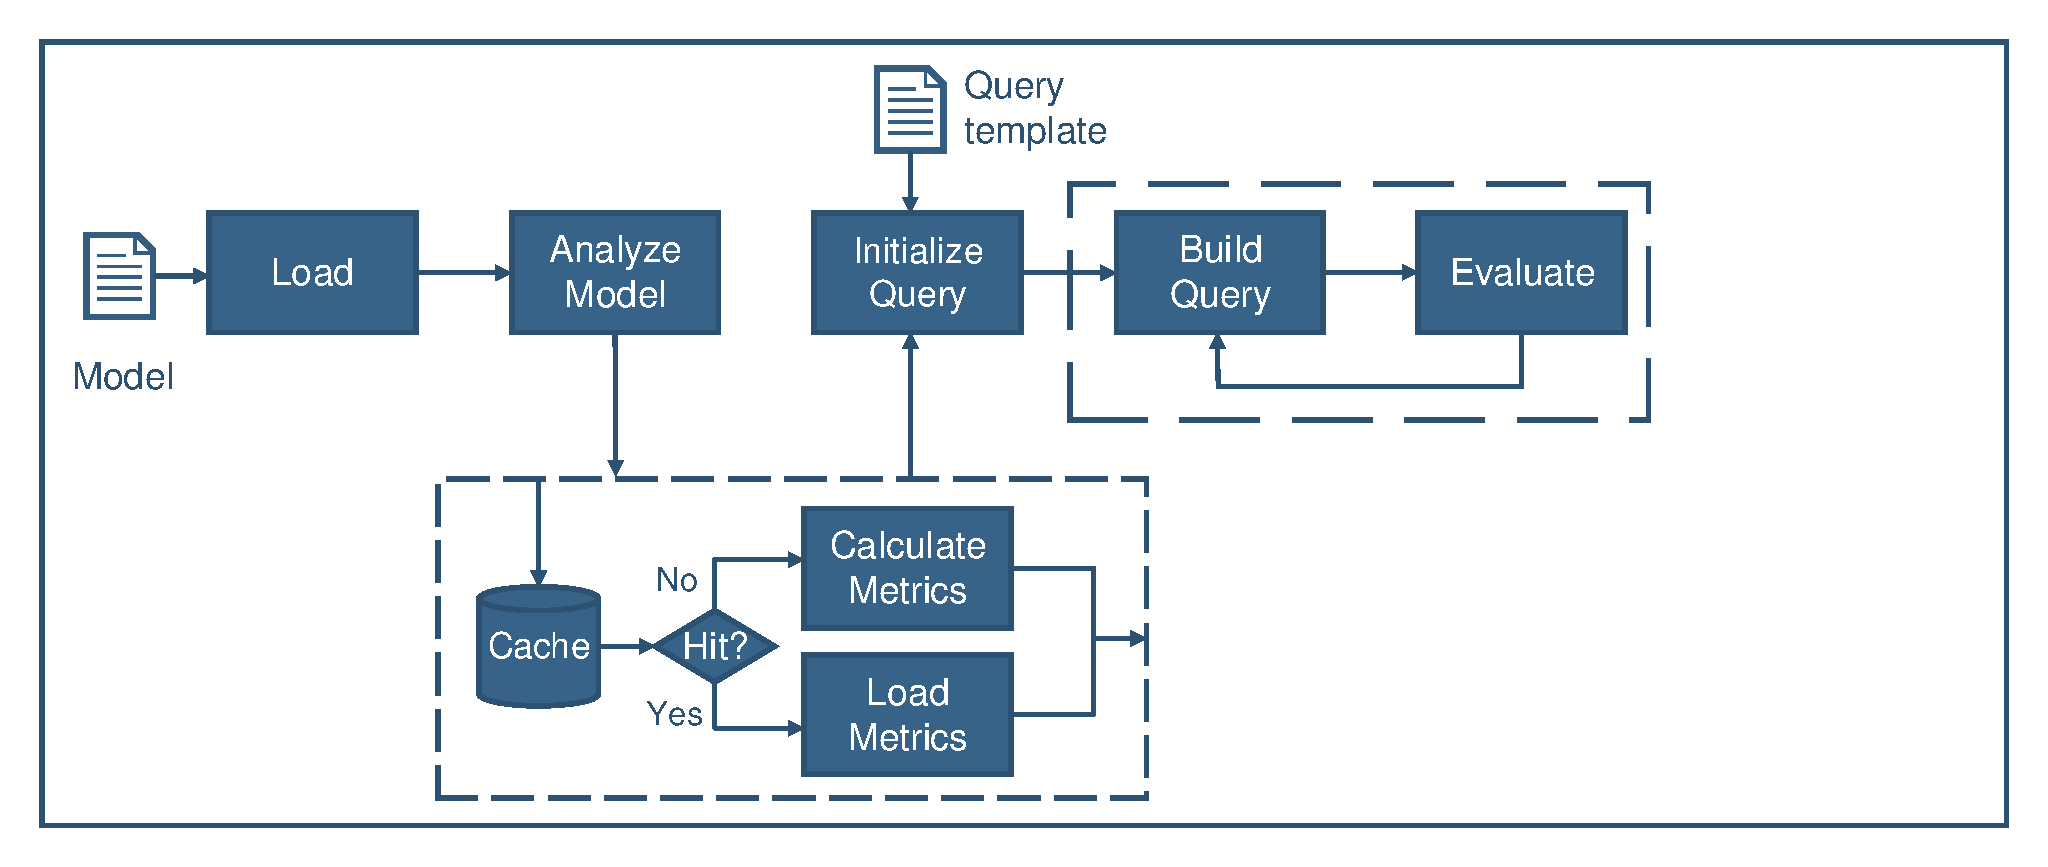
\includegraphics[width=150mm, keepaspectratio]{figures/workflow.pdf}
	\caption{The workflow of the HG Benchmark.}
	\label{fig:mondo_map_workflow}
\end{figure}

The workflow of the HG Benchmark is represented in Figure \ref{fig:mondo_map_workflow}. After loading the model, the framework calculates the model related metrics. Due to the fact that in the current phase of our research we do not consider model transformations, therefore, a particular model's metrics must be calculated only once in the beginning of the workflow. More importantly, different runs of the benchmark can utilize the previously calculated metrics that belong to the same model. As it can be observed in the model analysis phase, the solution is achieved by using a cache for the calculated metrics and reusing its content if possible.

The features in the \textsf{Initialize} and \textsf{Build Query} phases are strongly correlated. These two phases entail the creation of dynamic queries. The first one provides a default query definition that can be parameterized, and the second phase assembles a complete query for the evaluation, as it injects parameters or alters the entire syntax. The latter operation implies that entirely different queries can be executed in a sequence.

Last, the evaluation phase is responsible for executing the query. The \emph{build} and \emph{evaluate} phases can be repeated implying that more then one query can be evaluated in a sequence, even with different definitions.

\subsection{Metrics Calculation}
As we already emphasized, the \framework framework proposes two types of metrics. The first is the set of model descriptive metrics and the second relates to the query definitions. In the following, we introduce them and their calculations in the HG Benchmark.

\subsubsection{Model Metrics}
The model-based metrics are connected to graph metrics which appear in their naming conventions as well. Since we are concentrating on RDF tools in our work, we also define the corresponding interpretations. The metrics are listed hereunder.
%todo rdf and graph metrics
\begin{enumerate}
	\item{\textbf{Nodes:}} the number of nodes in the graph. In RDF, this equals to the number of unique subject and object values.
	\item{\textbf{Edges:}} the number of edges in the graph. Regarding RDF, this is equal to the number of predicates\footnote{With the consideration of \textsf{rdf:type} predicates, the number of edges metric represents the number of triples.} in the data.
	\item{\textbf{Maximum Degree:}} the maximum number of predicates per subjects.
	\item{\textbf{Average Degree:}} it is determined by calculating the degree of every existing node.
	\item{\textbf{Average Degree Distribution:}} denotes the probability that a randomly selected node’s degree is equal to the average degree.
	\item{\textbf{Higher Degree Distribution:}} the cumulative distribution of those nodes that have higher degrees than the average.
	\item{\textbf{Average Clustering Coefficient:}} this metric implies the calculation of clustering coefficient per every node.
	\item{\textbf{Average Shortest Path Length:}} the calculation of this metric is most expensive, hence, the framework searches a limited number (100) of shortest paths between randomly selected vertices and calculates their average length.
	\item{\textbf{Maximum Betweenness Centrality:}} the value of this metric is determined by the shortest paths. We count the occurrences of every intermediate node in the paths---by determining the betweenness centrality of the vertices---and normalize the values to the $[0,1]$ interval by dividing them with the number of visited nodes. Since the value of betweenness centrality is assigned to each node separately, we use the maximum of them.
\end{enumerate}

\subsection{Queries}

We investigate the performance of two queries in our HG Benchmark. The first one relates to the concept of \textit{shortest path}, and the second connects to the notion to investigating the \textit{spread of information} in the graphs.

\subsubsection{Shortest Path Query}

The SPARQL definition of the query is shown below:\\
\lstinputlisting{content/queries/transitive.sparql}

The query uses the \textsf{*} operator from SPARQL Property Paths~\cite{property_path} in the \textsf{(base:neighbor)*} predicate which means an arbitrary length of path with the \textsf{neighbor} predicates. The query is a parameterized query in which we inject two random identifiers instead the \textsf{ID} parameters. Finally, the query searches a path between those two nodes.

\subsubsection{Information Spread Query}
%todo mention spread of information in background betweenness
The query investigates the spread of information in the graph---by starting from a randomly chosen node---and it traverses the graph via the \textsf{neighbor} predicates to a three-hop distance. The concept of information spreading means how fast the information can be forwarded among the nodes in the graph, or in other words, how many vertices can be reached from a certain node.\\
The SPARQL definition of the query is shown below. As it can observed, in every new navigation we filter the previously found nodes to prevent the traversal of the same nodes again.

\lstinputlisting{content/queries/spread.sparql}

\subsection{Tools}

The tools used in this report are listed in Table \ref{tab:tools}. The last two columns illustrate whether the execution of our defined queries is feasible in the particular tool or not. As the table suggests, the first query cannot be evaluated in \textsf{4store}, since it does not support the usage of property paths.

\begin{table}[ht]
	\footnotesize
	\centering
	
	\begin{tabular}{ l c c c c c}
		\toprule
		Name & Implementation Language& Version & Query 1 & Query 2\\ 
		\midrule 
		AllegroGraph~\cite{allegro} & Allegro Common Lisp & 5.0.0  & \textbullet&  \textbullet \\ \hline
		Blazegraph~\cite{blaze} & Java  & 1.5.2 & \textbullet & \textbullet\\ \hline
		4store~\cite{4store} & C  & 1.1.5 & & \textbullet \\ \hline
		Jena~\cite{jena_api} & Java & 2.13.0 & \textbullet & \textbullet\\ \hline
		Sesame~\cite{sesame} & Java & 2.7.9 & \textbullet & \textbullet\\ \hline
		\bottomrule
	\end{tabular}
	\caption{The implemented tools in HG Benchmark}
	\label{tab:tools}
\end{table}


\subsection{Regression Analysis}

\subsubsection{MARS}



	
\chapter{Evaluation}

%\subsection{Design}

%Our design is constructed as follows. We generate different graph topologies with different densities and achieve a deviation in their %representative metrics, especially concentrating on the clustering coefficient, betweenness centrality and average shortest path. Our assumption is %that these metrics affect mostly and characterize the performance. We investigate the relationships between metrics and performance in the graphs %that contain the same number of nodes. 

\section{Benchmarking Environment}

The benchmarking environment involves a single machine that contains a quad-core Intel Xeon Processor L5420 (2.5 GHz) and 16 GBs of RAM. In order to alleviate disturbance of a running measurement and minimize the noise in the results, a bare metal 64-bit Ubuntu 14.04.2 LTS was installed. Additionally, Oracle JDK version 1.7.0 was used as the Java environment.


\section{Benchmark Configuration}

\paragraph{Topologies}

We generate five topologies for the measurements such as the scale-free model, hierarchical network and Watts-Strogatz models with different probability $p$ values as $0.1$, $0.01$ and $0.001$. Due to these configurations of $p$, we reach a deviation between Watts-Strogatz models and random graphs.\\ The topologies are generated via our uniform model generation approach (\ref{sec:uniform_generation}).
Every topology is generated five times with different densities that are adjusted to five different values based on the size of $K_n$ complete graphs found in the hierarchical network. These $K_n$ complete graphs are configured to $K_3$, $K_4$, $K_5$ $K_6$ and $K_7$.

\paragraph{Queries}
The queries are parameterized and executed for 20 times in a sequence on every graph. Furthermore, every measurement is repeated 4 times.

\paragraph{Model Size}

The configuration of the model sizes are shown in Table \ref{tab:graph_size} representing number of nodes and edges. The latter is given by an interval since we generate the graph with different densities.

\begin{table}[ht]
	\footnotesize
	\centering
	
	\begin{tabular}{ l c c c}
		\toprule
		Nodes & Min Edges & Max Edges \\ \hline
		%		\midrule 
		5~000 & 23~531 & 42~633\\ \hline
		10~000 & 49~140 & 89772\\ \hline	
		20~000 & 100656 & 185420\\ \hline
		40~000 & 209439 & 381435\\ \hline
		80~000 & 421110 & 800314\\ \hline
		\bottomrule
	\end{tabular}
	\caption{The number of nodes and edges in generated graphs.}
	\label{tab:graph_size}
\end{table}

\section{Samples}

In order to analyze the relationships between model metrics and performance of query evaluations, we create different samples of the measurements and investigate them respectively. The triple of a tool, query and a specific model size (number of nodes) defines a sample meaning that it includes the measurement results of one particular query per a tool based on a certain size of the models. As a result, the number of different samples is equal to the product of unique tools, queries and model sizes.

\subsection{Sample Size}
A sample includes the measurements executed on 5 different topologies, each of them appears 5 times in the sample with different densities that are configured between the various topologies equally. One sample contains 20 evaluations of a parameterized query. Every measurement is repeated 4 times in a sequence, however, we reject the first evaluation times and use the median of the remained measurements.\\
The dimensions in a sample and their occurrences are illustrated in Table \ref{tab:sample_size}. Since the triple of tool, query and model size defines a different sample, these values represent one value in a sample. As it can be observed, the sample size is equal to $500$.

\begin{table}[ht]
	\footnotesize
	\centering
	
	\begin{tabular}{ l c c c c c c || c }
		\toprule
		 & Tool & Query & Model Size & Query Evaluation & Topology  & Density & $\prod$\\ [5pt] \hline
%		\midrule 
		Occurrence & 1 & 1 & 1 & 20 & 5 & 5 & 500 \\ \hline
		\bottomrule
	\end{tabular}
	\caption{The dimensions and their occurrence in a sample.}
	\label{tab:sample_size}
\end{table}


\section{Model Analysis}

\subsection{Density}
One essential expectation was in our work to generate different graphs with the same number of nodes and edges. Figure \ref{fig:density} depicts the density of the topologies. The $x$-axis represents the sizes of the models, the $y$-axis shows the values belonging to density. Every column contains the information of one specific topology, furthermore, the different densities are separated by colours in the legend.
\begin{figure}[!ht]
	\centering
	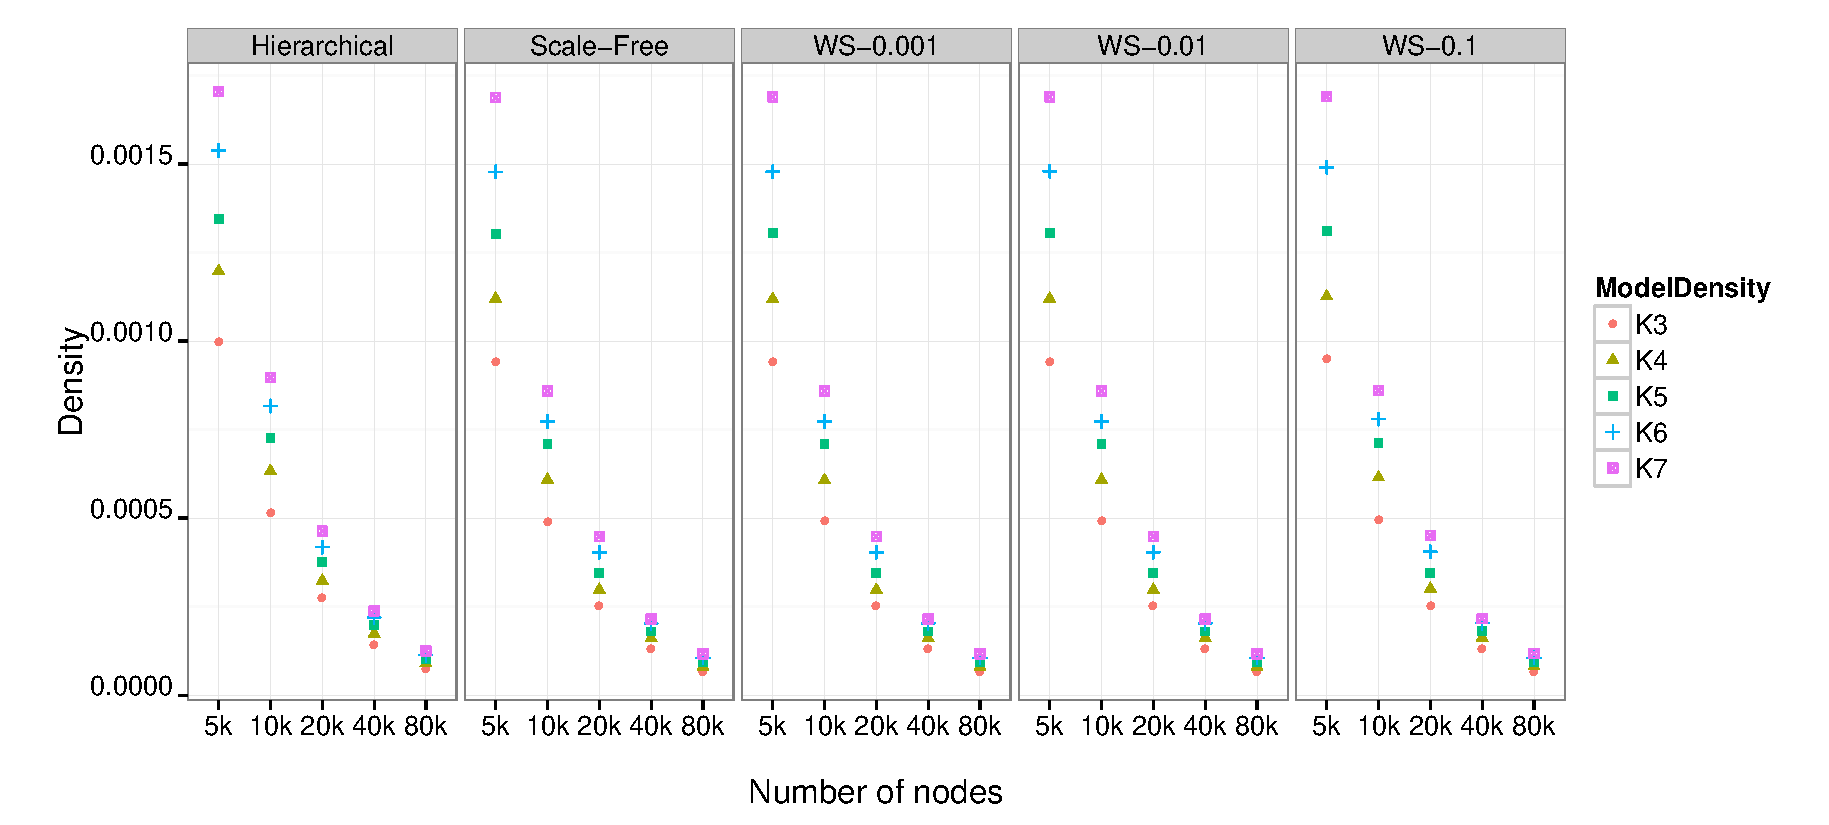
\includegraphics[width=160mm, keepaspectratio]{figures/density.pdf}
	\caption{The density of the graph topologies.}
	\label{fig:density}
\end{figure}

As it can be observed, the topologies with different networks have approximately the same density with the respect to the number of nodes, which implies an equality in the number of edges. A small deviation is shown between the hierarchical graph and the other topologies. This is explained by the fact that the recursive generation algorithm of the hierarchical network must be terminated before its end in order to obtain an arbitrary number of nodes. Hence, we can only estimate the amount of edges in the graph with a dispersion. The standard deviation of the densities is $1.11 \cdot 10^{-5}$, and divided by the maximum number of density we obtain 0.028, which means a 2.8\% difference between the topologies with respect to their density.

\subsection{Clustering Coefficient}

Our goal is to achieve a deviation in metric values per topologies such as the clustering coefficient metric. Figure \ref{fig:clustering_metric} depicts the average clustering coefficients in the topologies. The $x$-axis represents the number of nodes in the graphs, the $y$-axis denotes the values of the metric, furthermore, every value is separated by the topology in legend.\\
The plot shows how the values spread in the $0-1$ interval according to our early expectation (Section \ref{sec:topology_metric}). One topology has more corresponding metric value in the same size---\eg hierarchical---due to the fact that we generated 5 instances of every topology with different densities, which implies a different clustering coefficient metric per instance as well.

\begin{figure}[!ht]
	\centering
	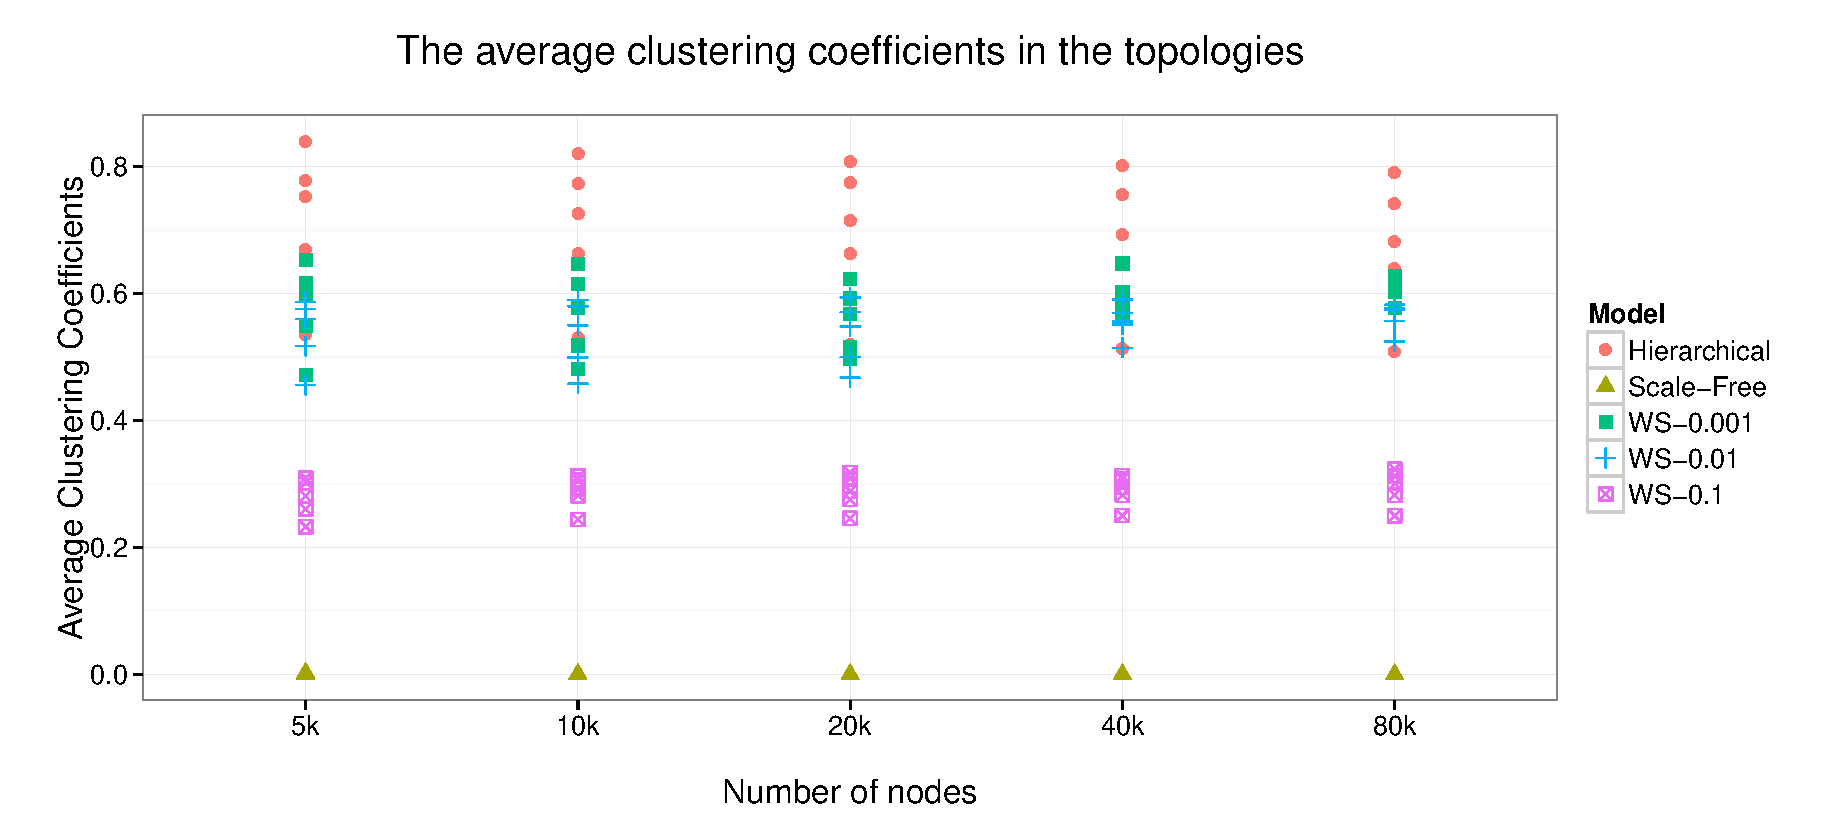
\includegraphics[width=160mm, keepaspectratio]{figures/clustering_metric.pdf}
	\caption{The average clustering coefficient in the graph topologies.}
	\label{fig:clustering_metric}
\end{figure}

\subsection{Shortest Path Length}

The average lengths of shortest paths in the topologies are demonstrated in Figure \ref{fig:betweenness_metric}. Easy to observe that as we decrease the $p$ probability in the Watts-Strogatz models (from $0.1$ to $0.001$) , the lengths of the shortest paths increase. This negative correlation shows the same results that we expected and can be explained by the operation of the generation algorithm belonging to the Watts-Strogatz model. As we increase the $p$ value, the algorithm rewires every edge with $p$ probability---\ie it deletes an edge and connects it to a new random node---and this entails a bigger interconnectivity in the graph showing a small-world property. On the contrary, a low $p$ value (\eg 0.001) modifies a subtle set of the edges, therefore, the graph still shows similar characteristics than a lattice graph with high average shortest path length.

\begin{figure}[!ht]
	\centering
	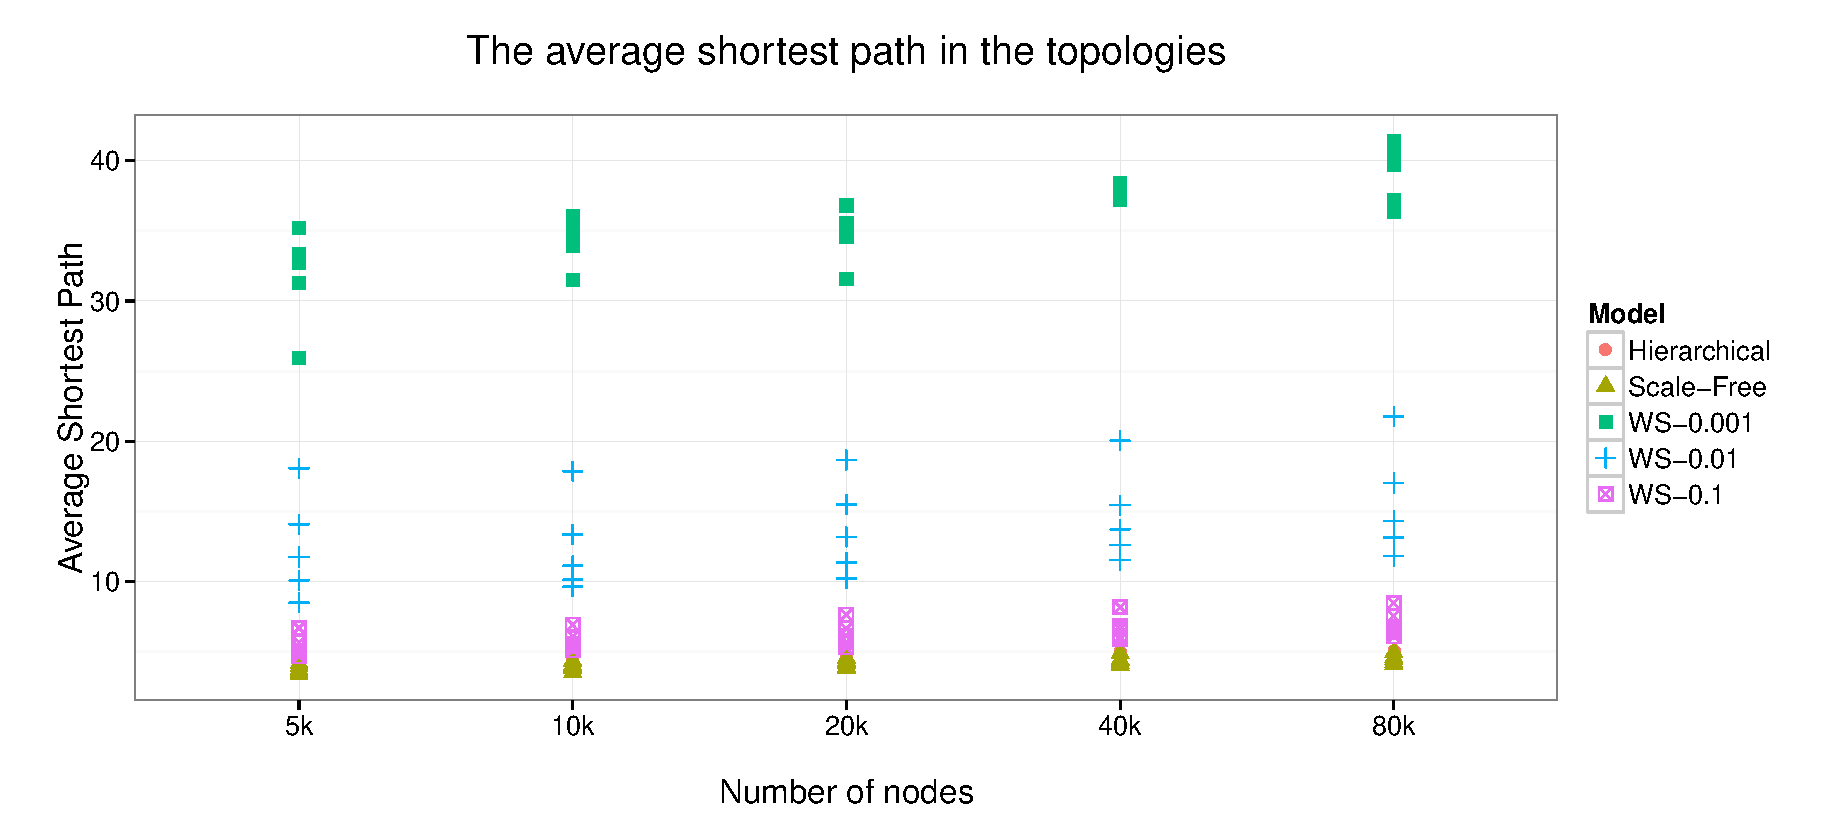
\includegraphics[width=160mm, keepaspectratio]{figures/avg_sp_metric.pdf}
	\caption{The average shortest path in the graph topologies.}
	\label{fig:avg_shortest_path}
\end{figure}

\subsection{Betweenness Centrality}

Figure \ref{fig:betweenness_metric} illustrates the betweenness centrality metric per topologies. Regarding this metric, we assumed a more significant deviation among the topologies, as we expected that the \emph{hubs}---the nodes with higher degrees---in scale-free models appear more times in the shortest paths implying a higher betweenness centrality. Instead, the WS-0.001 model shows higher values in this metric than the scale-free model except in the case of the largest graph.\\
A gap is observed between the hierarchical network and the other topologies due to the fact the center node in the hierarchical graph dominates the calculation of the betweenness centrality metric.

\begin{figure}[!ht]
	\centering
	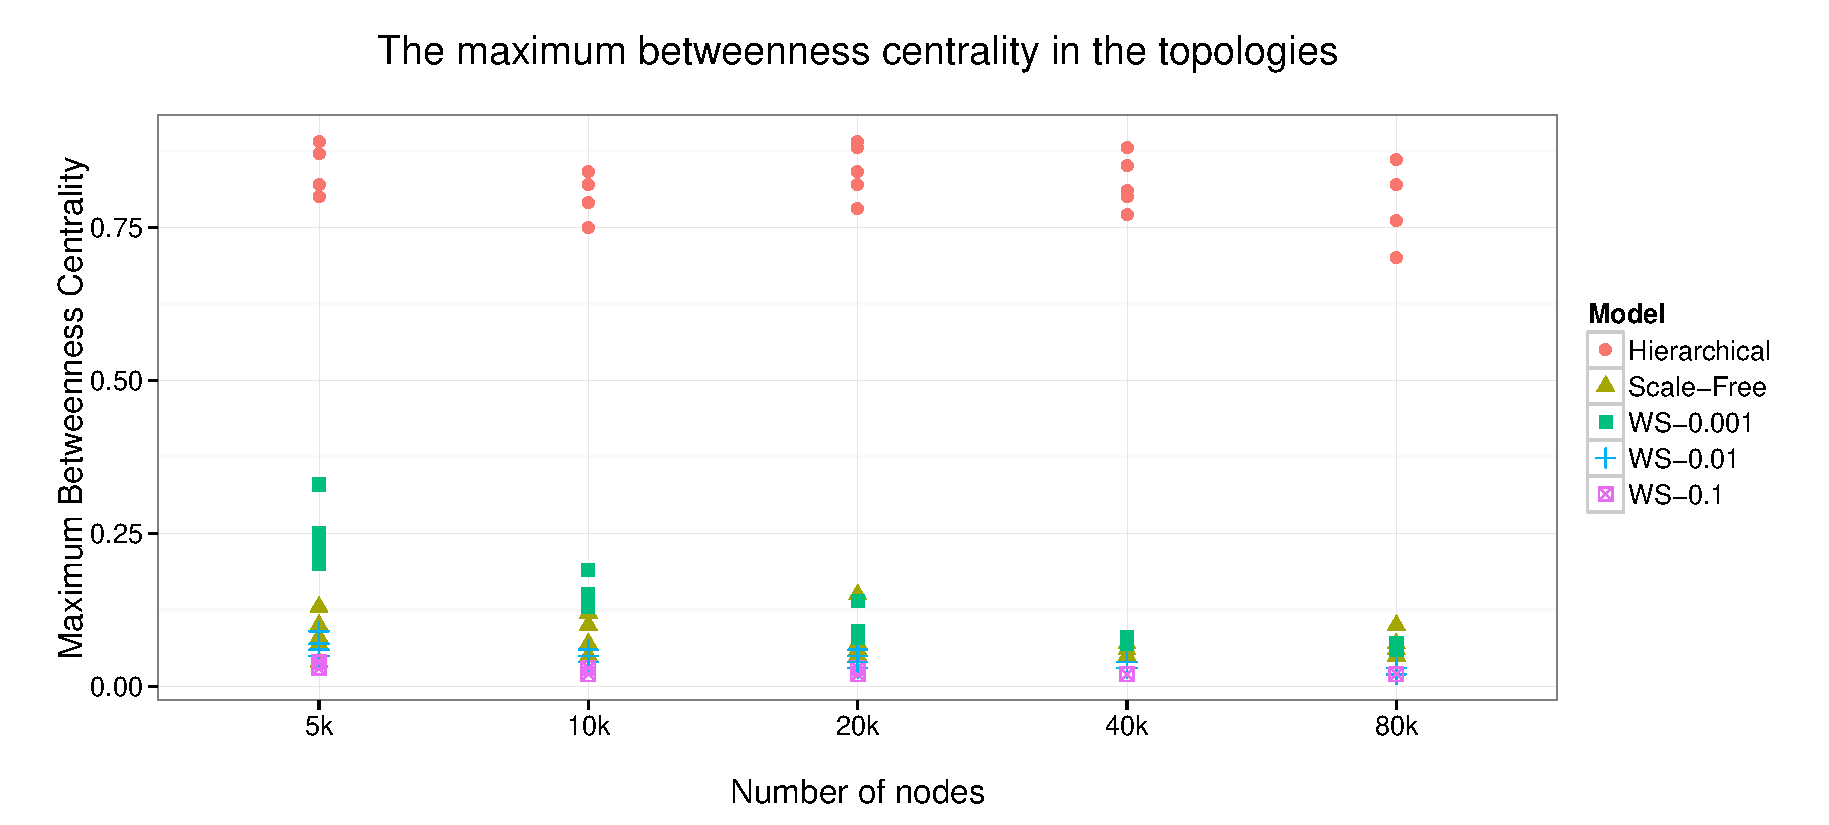
\includegraphics[width=160mm, keepaspectratio]{figures/betweenness_metric.pdf}
	\caption{The maximum betweenness centrality in the graph topologies.}
	\label{fig:betweenness_metric}
\end{figure}

\section{Performance Analysis}

\subsection{Hypothesis}

Our hypotheses about the results of query evaluations are the following.

\paragraph{Reachability Query}
Regarding the first query---Reachability---we assume that the larger clustering coefficients and higher degrees may cause a performance loss of the tools. If the graph has a higher clustering coefficient then there is a possibility that the execution of the query revisits a certain node more times via its neighbors. This implies that the evaluation contains more---unnecessary---navigations.\\
A node with higher degree also can affect the performance, since if the graph traversal visits this certain node with higher degree than there is a possibility that it also investigates its neighbors. Nodes with high degree typically appear in the scale-free models---the hubs---and the hierarchical networks---the center nodes.

The assumption comes naturally that the average shortest path length also can dominate the execution time. Among the different Watts-Strogatz models, the ones with lower $p$ values include a higher average shortest path metric, suggesting a growing in the evaluation time. However, considering the other topologies as well, it cannot be determined forward which specific characteristic dominates better.

\paragraph{Navigations Query}

The Navigations query searches nodes in three-hop distances starting from a random vertex. We believe that the nodes with higher degrees impact the performance mostly, namely, the center nodes in the hierarchical graph and the hubs in the scale-free models. We fundamental question is that whether our defined metrics are suitable to characterize the performance appropriately or not.

\subsection{Highlights of the Analysis}

For the performance analysis we created and measured 50 different samples, each of them contains 500 observations---\ie measurement results. In the following sections we do not intend to show the results in details of every sample, hence, we only concentrate on the samples that contain interesting or unexpected results.

\subsubsection{Blazegraph is highly sensitive to the average shortest path of the graph}

The measurement results of Blazegraph is illustrated in Figure \ref{fig:blazeq1}. The box plot~\cite{boxplot} shows the results in following dimensions. On the $x$-axis denotes the graph topologies and the $y$-axis represents the evaluation time in milliseconds on a logarithmic scale. Every column includes different results belonging to a specific model size.

\begin{figure}[!ht]
	\centering
	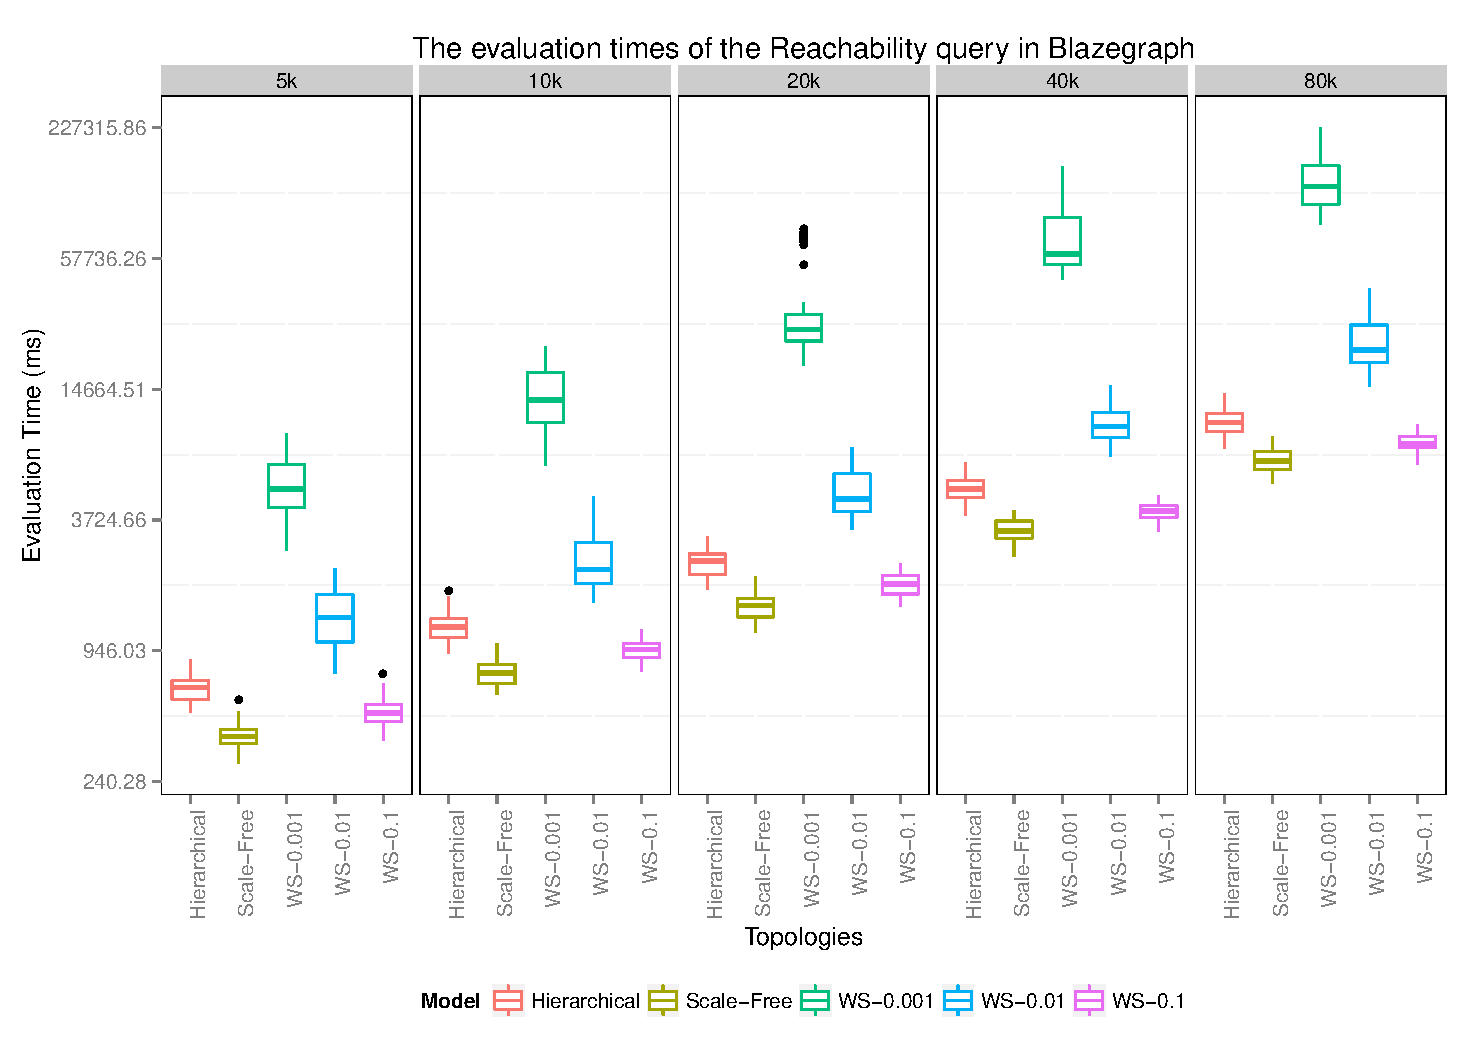
\includegraphics[width=160mm, keepaspectratio]{figures/blaze_q1.pdf}
	\caption{The measurement results of the Reachability query in Blazegraph.}
	\label{fig:blazeq1}
\end{figure}

The most important observation is the deviation in evaluation time among the topologies. Besides the execution times increases with respect to the number of nodes, the performance also varies among the networks being in the same size. A significant difference is shown between the Watts-Strogatz models (WS-$0.001$, WS-$0.01$) and the other networks.

The created regression models are listed in Table \ref{tab:regressions_blaze_a1}. Every measurement result and metric were normalized for the calculations, and the table includes the best fitted regression models on the measurements. In every case, the average shortest path metric seemed to be the best predictor. Regarding different model sizes, the value of adjusted R$^2$---\ie coefficient of determination---varies between 0.68 and 0.9 that show well-fitted regression models. 

\begin{table}[ht]
	\footnotesize
	\centering
	\begin{tabular}{ c c c c c}
		\toprule
		Model Size & Metric & Adjusted R$^2$& Regression Coefficient & P-value\\ \hline
		%		\midrule 
		5~000 & Avg Shortest Path & $0.9$ & 0.949 & $2.2 \cdot 10^{-16}$ \\ 
		10~000 & Avg Shortest Path & 0.8586 & 0.9268 & $2 \cdot 10^{-16}$ \\ 
		20~000 & Avg Shortest Path & 0.6807 & 0.8254 & $2.377 \cdot 10^{-16}$\\ 
		40~000 & Avg Shortest Path & 0.7647 & 0.8745 & $3.3\cdot 10^{-16}$ \\  
		80~000 & Avg Shortest Path & 0.7642 & 0.8745 & $3.3\cdot 10^{-16}$ \\  
		\bottomrule
	\end{tabular}
	\caption{The best fitted regression models of Blazegraph.}
	\label{tab:regressions_blaze_a1}
\end{table}

\subsubsection{Sesame is mostly unaffected by the topology of the model}

The evaluation results of Sesame are illustrated in Figure \ref{fig:sesame_q1}. As it can be observed, the optimization in Sesame is not sensitive to the different topologies, as the various characteristics of the networks still cause nearly the same evaluation time. A higher difference only occurs between the different model sizes. Interestingly, a small difference is also observable between the Watts-Strogatz models, as the $p$ values increases---implying the decrease of the average shortest path metric---the evaluation times still grow.\\
Due to the approximately equal results, we cannot create an appropriate well-fitted regression model for Sesame.

\begin{figure}[!ht]
	\centering
	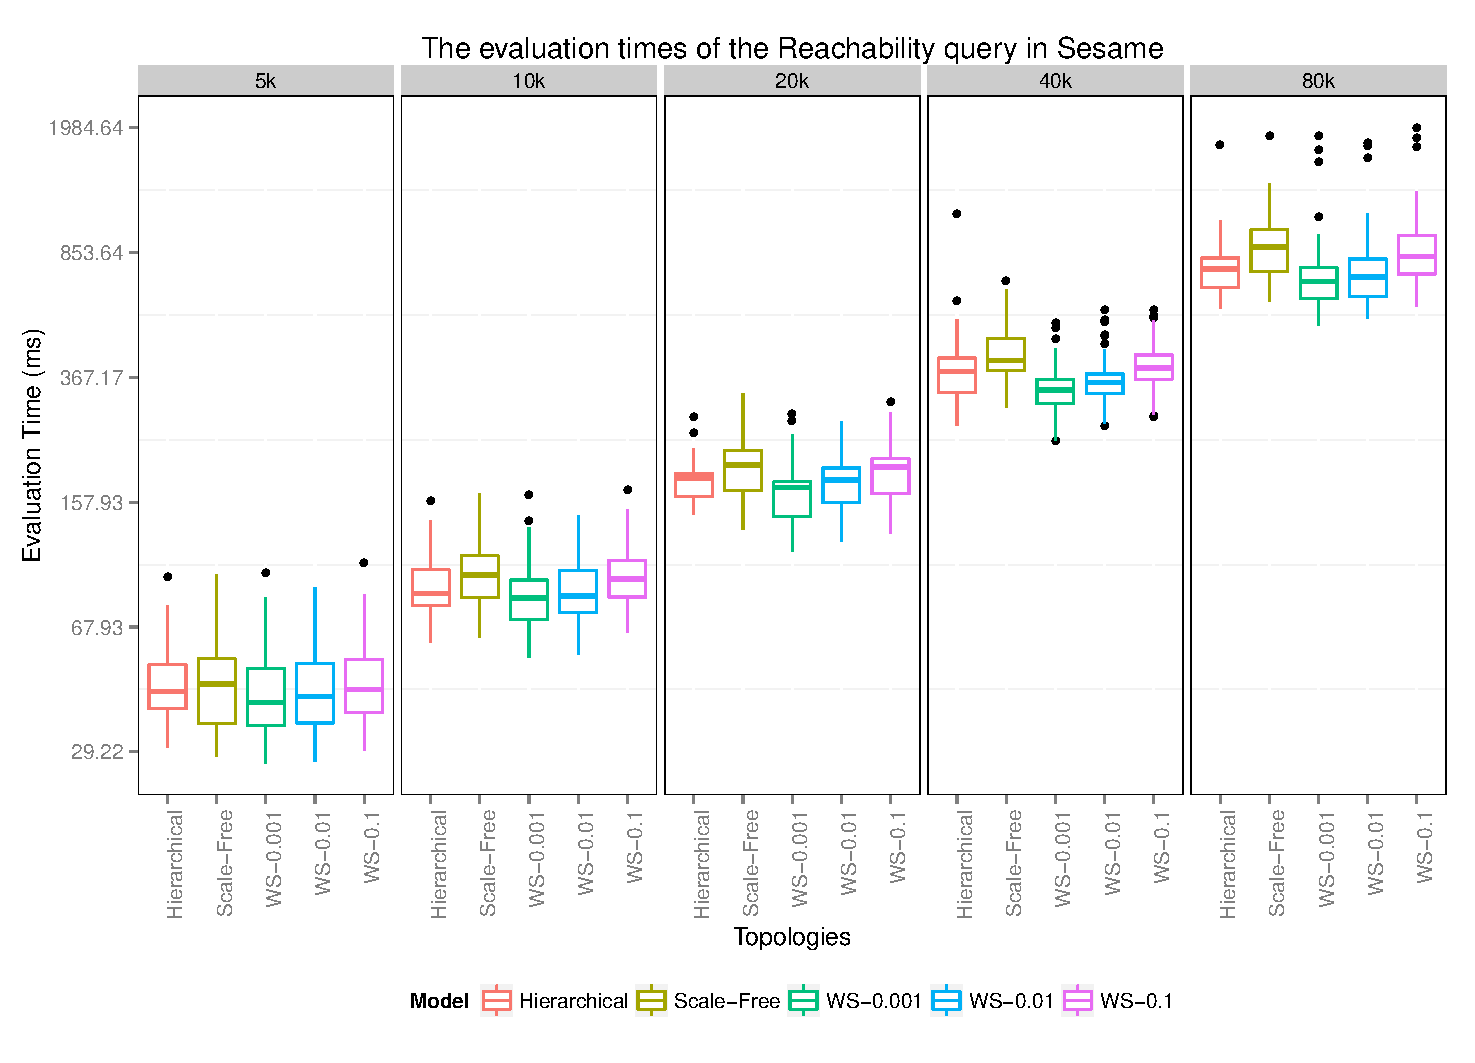
\includegraphics[width=160mm, keepaspectratio]{figures/sesame_q1.pdf}
	\caption{The measurement results of the Reachability query in Sesame.}
	\label{fig:sesame_q1}
\end{figure}

\subsubsection{The clustering coefficient does not influence the performance for the Reachability test}

Interesting to show that our assumption about the clustering coefficient metric is proved to be false. The adjusted R$^2$ values of the regression models containing the clustering coefficient are considerably small. In the case of Sesame, the adjusted R$^2$ is approximately 0.06 per different model sizes, and regarding Blazegraph, this value is equal to 0.13. Both of them indicate that the clustering coefficient has a minimal impact to the performance, in the light of these workloads.

\subsubsection{Negligible relationship between the hubs and the performance of the Reachability test}

The results of the Reachability query shows that the nodes which have significantly larger degrees do not affect the performance of the evaluations. At first sight, we would assume that the occurrence of hubs implies that the execution of the query must visits a significantly larger amount of nodes. Since, if the evaluation reaches a hub during the graph traversal than it possibly must visit its neighbors as well, causing a performance loss. However, in the case of Blazegraph, the Watts-Strogatz models with higher average shortest path lengths seem to be dominating, despite the fact that the same Reachability test in a hierarchical or scale-free network may visit more vertices than in the case of the WS models.

\subsubsection{Navigations on graphs are dominated by hubs}

The measurement results of the Navigation query is illustrated in Figure \ref{fig:fourstore_q2}. As we assumed, the hubs---\ie the significantly higher degree nodes---affect the performance of this query evaluation. A more interesting question is that whether our metrics can characterize this relationship appropriately or not. 

\begin{figure}[!ht]
	\centering
	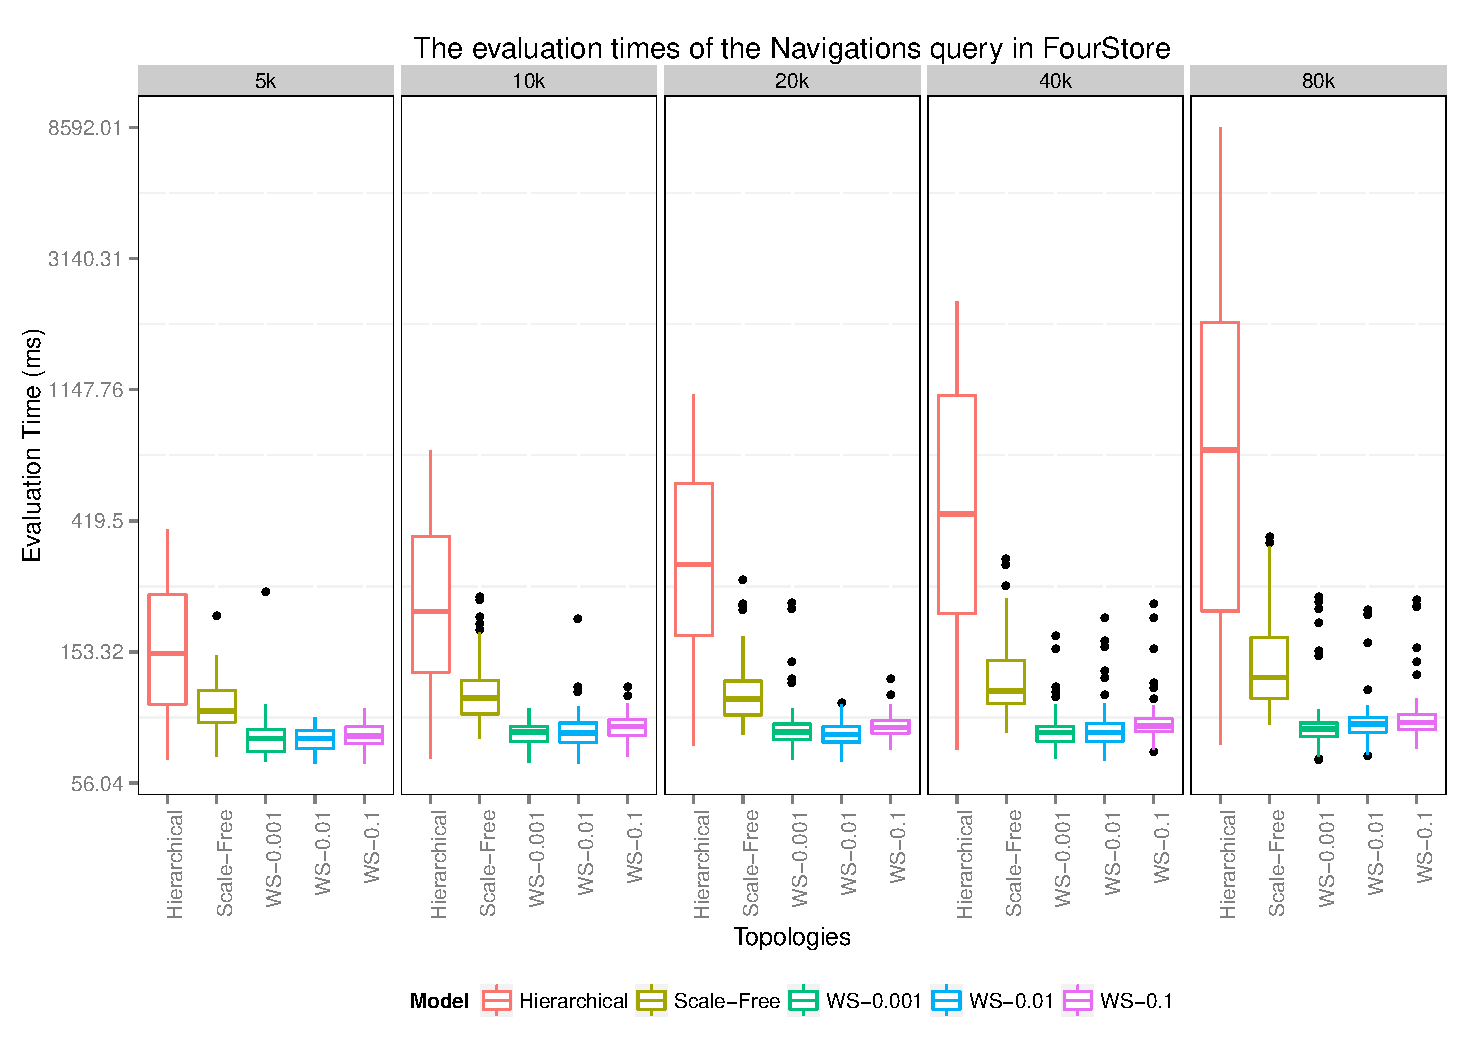
\includegraphics[width=160mm, keepaspectratio]{figures/4store_q2.pdf}
	\caption{The measurement results of the Navigations query in FourStore.}
	\label{fig:fourstore_q2}
\end{figure}

Our created regression models are shown in Table \ref{tab:regressions_4store_q2}. These are the ones that provided the best fit to the data including the betweenness centrality and maximum degree metric. The main conclusion is that our metrics partly can characterize the relationship, since the adjusted R$^2$ values vary between the 0.4396 and 0.5228 interval.
\begin{table}[ht]
	\footnotesize
	\centering
	\begin{tabular}{ c c c c c}
		\toprule
		Model Size & Metrics & Adjusted R$^2$ &  P-value\\ \hline
		%		\midrule 
		5~000 & Betweenness + Maximum Degree & 0.5228 & $2.2 \cdot 10^{-16}$ \\ 
		10~000 & Betweenness + Maximum Degree & 0.5204 & $2.2 \cdot 10^{-16}$ \\ 
		20~000 & Betweenness + Maximum Degree & 0.5125 & $2.2 \cdot 10^{-16}$\\ 
		40~000 & Betweenness + Maximum Degree & 0.4815 & $2.2\cdot 10^{-16}$ \\  
		80~000 & Betweenness + Maximum Degree & 0.4396 & $2.2\cdot 10^{-16}$ \\  
		\bottomrule
	\end{tabular}
	\caption{The best fitted regression models of Fourstore..}
	\label{tab:regressions_4store_q2}
\end{table}

As far as the other tools are concerned, such as Sesame and Blazegraph, the same metrics can be used to obtain the best fitted regression, and the adjusted R$^2$ values vary between the 0.4018 and 0.5173 interval. These results also show that only these two metrics were not adequate to characterize the performance properly regarding these workloads and samples.

\section{Conclusions}

\paragraph{Model Generation}
We showed that our model generation approach was able to construct different topologies with the same density with respect to the same number of nodes. As it was illustrated, the clustering coefficient and average shortest path length metrics were deviated appropriately among the topologies. Unfortunately, the betweenness centrality metric seemed to be dominated by the hierarchical network, and it also showed a significantly lower value in the scale-free models, than we originally expected. 

\paragraph{Performance}
The measurement results illustrated that the different internal structure of the graphs are able to cause a deviation in evaluation time, regarding the Reachability and Navigations query as well. In the first query, Blazegraph seems to be sensitive to the average shortest path length metric, on the contrary, the performance of Sesame is not affected by the topologies regarding these workloads.

\paragraph{Hierarchical Graph}

The analysis of the topologies show that the hierarchical graph has significantly different descriptive metrics than the other topologies, furthermore, our measurement results of the Navigation query also imply that the hierarchical network is overly dominating to the performance by comparing with the other networks. Our generation technique also showed that---by relying on the hierarchical graph---we cannot achieve an arbitrary density in the graph which is possible with the generation algorithms of the other topologies. We had to adapt the other networks to the limitations of the hierarchical graph. As a conclusion, the hierarchical graph is not capable to be used in our framework in the future due to its limitations.


	\chapter{Summary}



\pagenumbering{roman}
%\setcounter{page}{\value{romanPage}}


% Acknowledgements
%~~~~~~~~~~~~~~~~~~~~~~~~~~~~~~~~~~~~~~~~~~~~~~~~~~~~~~~~~~~~~~~~~~~~~~~~~~~~~~~~~~~~~~
	%----------------------------------------------------------------------------
\chapter*{\koszonetnyilvanitas}\addcontentsline{toc}{chapter}{\koszonetnyilvanitas}
%----------------------------------------------------------------------------



% List of Figures, Tables
%~~~~~~~~~~~~~~~~~~~~~~~~~~~~~~~~~~~~~~~~~~~~~~~~~~~~~~~~~~~~~~~~~~~~~~~~~~~~~~~~~~~~~~
	\listoffigures\addcontentsline{toc}{chapter}{\abrakjegyzeke}
	\listoftables\addcontentsline{toc}{chapter}{\tablazatokjegyzeke}


% Bibliography
%~~~~~~~~~~~~~~~~~~~~~~~~~~~~~~~~~~~~~~~~~~~~~~~~~~~~~~~~~~~~~~~~~~~~~~~~~~~~~~~~~~~~~~
%todo check and delete the bullshit from bib
	\bibliography{bib/mybib}
	\addcontentsline{toc}{chapter}{\irodalomjegyzek}

% Appendix
%~~~~~~~~~~~~~~~~~~~~~~~~~~~~~~~~~~~~~~~~~~~~~~~~~~~~~~~~~~~~~~~~~~~~~~~~~~~~~~~~~~~~~~
	\begin{figure}[!ht]
	\centering
	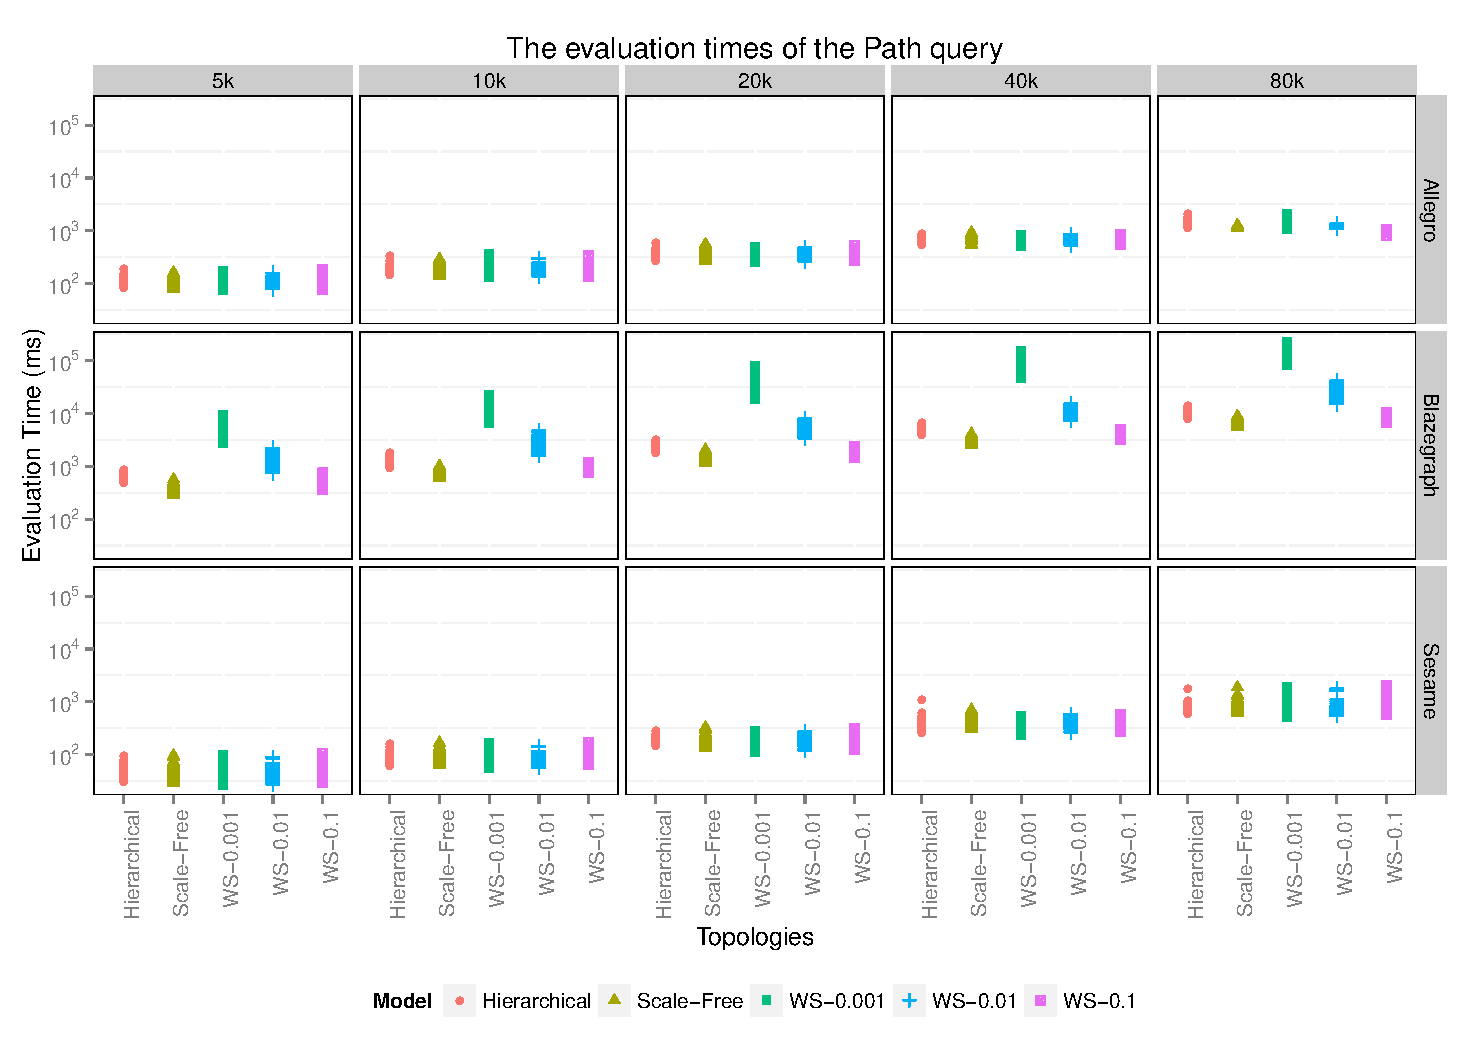
\includegraphics[width=160mm, keepaspectratio]{figures/query1_all.pdf}
	\caption{The measurement results of the Reachability query.}
	\label{fig:query1}
\end{figure}


\label{page:last}
\end{document}
